% !TeX encoding = UTF-8
% !TeX root = diplom.tex
% !TeX program = xelatex
% !TeX spellcheck = uk

\documentclass[a4paper,fontsize=14bp,ukrainian]{extreport}

%%%%%%%%%%%%%%%%%%%%%%%%%%%%%
% INCLUDE STRUCTURE .TeX FILE
%%%%%%%%%%%%%%%%%%%%%%%%%%%%%
%
% ПРЕАМБУЛА ДЛЯ ОФОРМЛЕНИЯ СОГЛАСНО
% ДСТУ3008:2015
%

\nonstopmode
%\usepackage{extsizes}

%\usepackage{cmap} % для кодировки шрифтов в pdf
\usepackage{lmodern}
\usepackage{calc} % калькулятор (операторы +- и т.п.)
\usepackage{scrextend}
\usepackage[no-math]{fontspec} % костыль
\usepackage{mathspec}
\usepackage{xunicode,xltxtra} % не мешает вроде
\usepackage{mathptmx}


% ПОЛИГЛОССИЯ
\usepackage{polyglossia} % на замену babel
\setmainlanguage{ukrainian}
\defaultfontfeatures{Mapping=tex-text} % чтобы работали "---" и прочее
\setotherlanguages{english, russian}
\newfontfamily\cyrillicfont[Script=Cyrillic]{Times New Roman}
\newfontfamily\cyrillicfonttt[Script=Cyrillic]{Times New Roman}

% СТАВИМ ШРИФТЫ
\setmainfont[Scale=1]{Times New Roman} % .976
\setmathfont(Digits,Latin,Greek)[Scale=1, Numbers={Lining,Proportional}]{Times New Roman}
\setmonofont{Times New Roman}
\linespread{1.5} % 1.464
% делаем чтобы запятые в формулах были тоже таймс нью роман
%\usepackage[output-decimal-marker=\textrm{,}]{siunitx}
%\renewcommand\materialfont{\sffamily\fontsize{7pt}{\baselineskip}\selectfont}
\usepackage{siunitx}
\sisetup{
  list-final-separator = { і },
  list-pair-separator  = { і },
  range-phrase         = { до },
  output-decimal-marker = {,},
  per-mode              = symbol,
  detect-weight=true,
  detect-family=true,
  group-digits = integer,
  group-minimum-digits = 3,
  group-separator = \text{~}
}
\DeclareSIUnit\gpa{\text{ГПа}}
\DeclareSIUnit\mkm{\text{мкм}}
\DeclareSIUnit\mal{\text{разів}}
\DeclareSIUnit\sec{\text{с}}
\DeclareSIUnit\kilog{\text{кг}}
\DeclareSIUnit\degree{\degree}
\DeclareSIUnit\mkomm{\text{мкОм$\cdot$м}}
\DeclareSIUnit\grn{\text{грн}}

\usepackage{icomma}
\begingroup
\lccode`\~`\,\lowercase{\endgroup
\def~{\mathpunct{\textrm{,}}}}

%%%%%%%%%%%%%%%%%%%%%%%%%%%%%%%%%%%%%%%%%%%%%%%%%%%%%%%%%%%%%%%%%%%%%%%%%%%%%%%%%%%

\usepackage{array}
\usepackage{graphicx} % для вставки картинок
\let\varTheta\undefined %КОСТЫЛЬ!!!
\usepackage{amsfonts,amsmath,amsthm} % математические дополнения от АМС
\usepackage{indentfirst} % отделять первую строку раздела абзацным отступом тоже
\usepackage[usenames,dvipsnames]{color} % названия цветов
\usepackage{makecell}
\usepackage{multirow} % улучшенное форматирование таблиц
%\usepackage{ulem} % подчеркивания
\usepackage{longtable} %длинные таблицы
\usepackage{ragged2e}
\usepackage{float}
\usepackage{pdfpages}
\usepackage[table]{xcolor}
\usepackage[obeyDraft]{todonotes}
%%%%%%%%%%%%%%%%%%%%%%%%%%
% КОЛОНТИТУЛЫ
%%%%%%%%%%%%%%%%%%%%%%%%%%

\usepackage{fancyhdr}
\pagestyle{fancy}
\fancyhf{}
\fancyhead[R]{\fontfamily{\familydefault}\fontsize{14pt}{14pt}\selectfont\thepage}
\fancyheadoffset{0mm}
\fancyfootoffset{10mm}
\setlength{\headheight}{17pt}%17pt
\renewcommand{\headrulewidth}{0pt}
\renewcommand{\footrulewidth}{0pt}
\fancypagestyle{plain}{%
  \fancyhf{}
  \rhead{\fontfamily{\familydefault}\fontsize{14pt}{14pt}\selectfont\thepage}}
%\setcounter{page}{} % начать нумерацию страниц с №5

%%%%%%%%%%%%%%%%%%%%%%%%%%
% ПОДПИСИ К РИСУНКАМ
%%%%%%%%%%%%%%%%%%%%%%%%%%

\usepackage[tableposition=top]{caption}
\usepackage{subcaption}
\DeclareCaptionLabelFormat{gostfigure}{Рисунок #2}
\DeclareCaptionLabelFormat{gosttable}{\hspace{0.75cm}Таблиця #2}
\DeclareCaptionLabelFormat{gostlisting}{\hspace{0.75cm}Лістинг #2}
\DeclareCaptionLabelSeparator{gost}{~---~}
\captionsetup{labelsep=gost}
\captionsetup[table]{%
  format=plain,
  justification=justified,%width=\linewidth,
  indention=0cm,
  font={stretch=1.464},
  singlelinecheck=false,
  labelformat=gosttable}

\captionsetup[lstlisting]{%
  format=plain,
  justification=justified,%width=\linewidth,
  indention=0cm,
  font={stretch=1.464},
  singlelinecheck=false,
  labelformat=gostlisting}

\captionsetup[figure]{%
  labelformat=gostfigure,
  indention=0cm,
  justification=centering,
  margin={0cm,14pt},
  font={stretch=1.464},
  indention=0cm}

\setlength{\textfloatsep}{0pt}
\setlength{\floatsep}{10pt}
\setlength{\intextsep}{10pt}
\setlength{\abovecaptionskip}{5pt}
\setlength{\belowcaptionskip}{-5pt}

\newcommand\fnote[1]{%
\justify
\setstretch{1.464}
{\hspace{1.25cm}#1}
}

\renewcommand{\thesubfigure}{\asbuk{subfigure}}

%%%%%%%%%%%%%%%%%%%%%%%%%%
% МЕЛОЧИ
%%%%%%%%%%%%%%%%%%%%%%%%%%
\parindent=1.25cm
\usepackage{ulem}
\usepackage{gensymb}
\usepackage{setspace}
%\usepackage[nodisplayskipstretch]{setspace}
\newcommand{\cels}{~${}^{\circ}C$}
\newcommand{\signline}{\rule{1.25in}{.5pt}}
\newcommand{\inputdateblank}{%
{,,}\rule{0.7cm}{.5pt}{\/``}\enspace\hrulefill~\the\year~р.}
%\newdateformat{mydate}{,,\underline{\THEDAY}\/``~\underline{\THEMONTH}~\THEYEAR~p.}

\newenvironment{eqitemize}
  {\itemize[label=,leftmargin=\widthof{де\enspace}]}
  {\enditemize}

%выключаем переносы и делаем выравнивание текста Word-like
\tolerance=1
\emergencystretch=\maxdimen
\hyphenpenalty=10000
\hbadness=10000


\usepackage[bookmarks=true,
            xetex,
            unicode=true]{hyperref}
%\usepackage{bookmark}
%\PassOptionsToPackage{unicode}{hyperref}
%\PassOptionsToPackage{naturalnames}{hyperref}
\hypersetup{
final=true,
 colorlinks,
  citecolor=black,
  filecolor=black,
  linkcolor=black,
  urlcolor=black}

\expandafter\def\expandafter\normalsize\expandafter{%
    \normalsize
    \setlength\abovedisplayskip{2pt}
    \setlength\belowdisplayskip{2pt}
    \setlength\abovedisplayshortskip{2pt}
    \setlength\belowdisplayshortskip{2pt}
}
%%%%%%%%%%%%%%%%%%%%%%%%%%
% ЛИСТИНГИ
%%%%%%%%%%%%%%%%%%%%%%%%%%
\usepackage{listings}

\lstset{% general command to set parameter(s)
  breaklines=true,
  inputencoding=utf8,
  %extendedchars=\true,
  frame=single,
  basicstyle=\linespread{1}\footnotesize,      % print whole listing small
  keywordstyle=\color{black}\bfseries\underbar,
  % underlined bold black keywords
  %identifierstyle=,           % nothing happens
  commentstyle=\color{gray}, % white comments
  %stringstyle=\ttfamily,      % typewriter type for strings
  showstringspaces=true,
  showspaces=false,
  %numbers=left,
  %stepnumber=1,
  %firstnumber=1,
  tabsize=2,
  caption=\lstname
  %numberfirstline=true
}

\renewcommand{\lstlistingname}{Лістинг}

%%%%%%%%%%%%%%%%%%%%%%%%%%
% ОГЛАВЛЕНИЯ
%%%%%%%%%%%%%%%%%%%%%%%%%%
\usepackage{titlesec}

\titleformat{\chapter}[hang]
{\filcenter}
%{\MakeUppercase{\chaptertitlename} \thechapter}
{\bfseries\thechapter}
{8pt}
{\bfseries}{}

\titleformat{\section}[block]
{\normalsize\bfseries}
{\thesection}
{1em}{}

\titleformat{\subsection}[block]
{\normalsize\bfseries}
{\thesubsection}
{1em}{}

% Настройка вертикальных и горизонтальных отступов
\titlespacing*{\chapter}{0pt}{-30pt}{30pt}
\titlespacing*{\section}{\parindent}{*4}{*4}
\titlespacing*{\subsection}{\parindent}{*4}{*4}

%%%%%%%%%%%%%%%%%%%%%%%%%%
% LIKECHAPTER
%%%%%%%%%%%%%%%%%%%%%%%%%%
\newcommand{\empline}{\mbox{}\newline}
\newcommand{\likechapterheading}[1]{%
  \begin{center}
    \textbf{#1}
  \end{center}
  \vspace{15pt} %УЖЕ ПОДПРАВИЛ БОЛЕЕ-МЕНЕЕ
  %\empline
}

\makeatletter
\renewcommand{\@dotsep}{1}
\newcommand{\l@likechapter}[2]{{\@dottedtocline{0}{0pt}{0pt}{#1}{#2}}}
\providecommand*{\toclevel@likechapter}{10}
\makeatother

\newcommand{\likechapter}[1]{
  \newpage
  \pdfbookmark[0]{#1}{#1}
  \likechapterheading{#1}
  \addcontentsline{toc}{likechapter}{#1}
  }

%%%%%%%%%%%%%%%%%%%%%%%%%%
% ПРИЛОЖЕНИЯ
%%%%%%%%%%%%%%%%%%%%%%%%%%
\usepackage[title]{appendix}

\titleformat{\paragraph}[display]
{\filcenter}
{\thechapter}
{8pt}
{\hspace{1.4in} ДОДАТОК \thechapter \newline \bfseries}{}
\titlespacing*{\paragraph}{0pt}{0pt}{-40pt}

\newcommand{\append}[1]{%
  \newpage
  %\stepcounter{chapter}%\chaptermark{#1}
  \refstepcounter{chapter}
  \pdfbookmark[0]{ДОДАТОК~\thechapter~#1}{ДОДАТОК~\thechapter~#1}
  \paragraph{#1}
  \empline
  \addcontentsline{toc}{likechapter}{ДОДАТОК~\thechapter~\;#1}
}

%%%%%%%%%%%%%%%%%%%%%%%%%%
% ЗМІСТ
%%%%%%%%%%%%%%%%%%%%%%%%%%
\usepackage{tocloft}
\tocloftpagestyle{empty}
\renewcommand{\cfttoctitlefont}{\hspace{0.435\textwidth} \bfseries\MakeUppercase}
\renewcommand\cftchappagefont{\normalfont}
\renewcommand{\cftbeforetoctitleskip}{-1em}
\renewcommand{\cftaftertoctitle}{\mbox{}\hfill \\ \mbox{}\hfill{%\footnotesize Стор.
             }\vspace{-2.5em}}
\renewcommand{\cftchapleader}{\cftdotfill{\cftdotsep}}
\renewcommand{\cftchapfont}{}
%\renewcommand{\cftsecfont}{\hspace{0pt}} % было 31pt
%renewcommand{\cftsubsecfont}{\hspace{0pt}} % было 11pt
\renewcommand{\cftbeforechapskip}{0em}
%\renewcommand{\cftafterchapskip}{1em}
\renewcommand{\cftparskip}{-1mm}
\renewcommand{\cftdotsep}{1}

%\renewcommand{\cftchapnumwidth}{32pt}
%\setlength{\cftchapindent}{-32pt}

\setcounter{tocdepth}{2} % задать глубину оглавления — до section включительно

%%%%%%%%%%%%%%%%%%%%%%%%%%
% ПОЛЯ
%%%%%%%%%%%%%%%%%%%%%%%%%%
\usepackage{geometry}
\geometry{left=2.5cm}
\geometry{right=1cm}
\geometry{top=2cm}
\geometry{bottom=2cm}

%%%%%%%%%%%%%%%%%%%%%%%%%%
% СПИСКИ
%%%%%%%%%%%%%%%%%%%%%%%%%%
\usepackage{enumitem}
\makeatletter
\AddEnumerateCounter{\asbuk}{\@asbuk}{м)}
\makeatother
\setlist{nolistsep,leftmargin=\widthof{---\enspace}+1.25cm}
%\setlist{}
\renewcommand{\labelitemi}{---}
\renewcommand{\labelenumi}{\asbuk{enumi})}
\renewcommand{\labelenumii}{\arabic{enumii})}

%%%%%%%%%%%%%%%%%%%%%%%%%%
% СПИСОК ЛИТЕРАТУРЫ
%%%%%%%%%%%%%%%%%%%%%%%%%%
%\usepackage{gost}
\usepackage[square,numbers,sort&compress]{natbib}
%\renewcommand{\bibnumfmt}[1]{#1.\hfill} % нумерация источников в самом списке — через точку
\renewcommand\bibnumfmt[1]{\hphantom{99.}\llap{#1.}}
\renewcommand{\bibsection}{\likechapter{СПИСОК ВИКОРИСТАНИХ ДЖЕРЕЛ}} % заголовок специального раздела
\setlength{\bibsep}{0pt}
\bibliographystyle{ugost2003}

\makeatletter
\newcommand\thefontsize[1]{{#1 The current font size is: \f@size pt\par}}
\makeatother

\graphicspath{{./figures/}}
\hypersetup{pdfauthor={студент ІФФ групи ФМ-31 Богомаз Р.Д.},
pdftitle={Створення функцiональних покриттiв на сталi~45 пошаровим електроiскровим легуванням хромом, вольфрамом та графiтом},
pdfsubject={Дипломна робота},
pdfkeywords={ЕЛЕКТРОІСКРОВЕ ЛЕГУВАННЯ} {ПОКРИТТЯ} {ВОЛЬФРАМ} {ХРОМ} {ГРАФІТ}}
%%%%%%%%%%%%%%%%%%%%%%%%%%%%%

%%%%%%%%%%%%%%%%%%%%%%%%%%%%%
% ДОКУМЕНТ
%%%%%%%%%%%%%%%%%%%%%%%%%%%%%
\begin{document}

%\includepdf[]{title.pdf}
%\includepdf[pages={1,2}]{task.pdf}


\setcounter{page}{4}

\chapter*{РЕФЕРАТ}
\thispagestyle{empty}
Дипломна робота: 77~с., 28~рис., 13~табл., 2~дод., 34~джерел.\vspace{5mm}
%TODO: need to automate counting of pages and other counters

ЕЛЕКТРОІСКРОВЕ ЛЕГУВАННЯ, ПОКРИТТЯ, ВОЛЬФРАМ, ХРОМ, ГРАФІТ.\vspace{5mm}

Об'єкт дослідження~---~поверхневі шари сталі~45 з нанесеними покриттями електроіскровим легуванням.

Мета роботи --- Дослідження структури, фазового складу та властивостей покриттів одержаних пошаровим нанесенням вольфраму, хрому та графіту на поверхню сталі~45 в процесі електроіскрового легування.

Методи дослідження --- гравіметричний, мікроструктурний, рентгеноструктурний, мікродюрометричний аналізи та випробування на зносостійкість.

Встановлена можливість створення функціональних покриттів на сталі~45 методом пошарового електроіскрового легування за схемами: Cr-W-C, W-Cr-C, W-C-Cr, C-Cr-W.

Виявлено зростання поверхневої мікротвердості в діапазоні від \SIrange{11.5}{18.9}{\gpa} через наявність в нанесених покриттях твердих розчинів на основі матеріалів електродів та карбідів WC, $\text{W}_2\text{C}$, $\text{Fe}_{3}\text{C}$, $\text{Cr}_{3}\text{C}_{2}$, $\text{CrC}$ в порівнянні з необробленою поверхнею.

Випробування в умовах сухого тертя за схемою ``площина по площині'' протягом 2~годин показали підвищення зносостійкості від \SIrange{3}{23}{\mal} в порівнянні з необробленим зразком сталі~45.

\chapter*{ABSTRACT}
\thispagestyle{empty}
Diploma work:  77~pages,  13~tables,  28~figures,  34~literary sources. \vspace{5mm}

ELECTRIC-DOPING, COATING, TUNGSTEN, CHROMIUM, GRAPHITE. \vspace{5mm}

Research object --- surface layers of steel~45 coated by electric-spark alloying.

Purpose --- research structure, phase composition and properties of coatings obtained by stratified application of tungsten, chromium and graphite on the surface of the steel~45 during electric-spark alloying.

Methods --- gravimetric, microstructural, X-ray, microhardness analyzes and durability tests.

It was verified the possibility of creating functional coatings on steel~45 by layered electric-doping schemes: Cr-W-C, W-Cr-C, W-C-Cr, C-Cr-W.

It was found growth of surface microhardness to range from 11,5~GPa to 18,9~GPa caused by coating of solid solutions based electrode material and carbides WC, $\text{W}_2\text{C}$, $\text{Fe}_{3}\text{C}$, $\text{Cr}_{3}\text{C}_{2}$, $\text{CrC}$ compared to untreated surface.

Tests in conditions of dry friction scheme ``plane to plane'' for 2~hours showed increasing durability from 3 times to 23 times compared to the untreated sample of steel~45.

\newpage
\tableofcontents
\thispagestyle{empty}

\likechapter{ПЕРЕЛІК СКОРОЧЕНЬ ТА УМОВНИХ ПОЗНАЧЕНЬ}
\label{likechap:abbrevation}

ЕІЛ --- електроіскрове легування

ВК --- вольфрамокобальтові твердосплави

ТК --- титановольфрамокобальтові твердосплави

ОКР --- області когерентного розсіювання

ЛШ --- легований шар

НДР --- науково-дослідна робота

ФЗП  --- фонд заробітної плати

В\textsubscript{С} --- єдиний соціальний внесок

С\textsubscript{М} --- транспортно-заготівельні витрати

С\textsubscript{інш} --- інші прямі невраховані витрати

Н\textsubscript{В} --- норматив відрахувань

Б --- бальна оцінка ефективності НДР


\likechapter{ВСТУП}
\label{likechap:intro}

Темпи сучасного виробництва висувають високі вимоги до деталей машин та інструменту щодо їх надійності та довговічності в процесі роботи у складних умовах. У зв’язку з цим, важливе завдання, поставлене перед матеріалознавцями, полягає у розробці нових сплавів з комплексом високих експлуатаційних властивостей, а також удосконаленні існуючих технологій обробки.

Для розв'язання існуючої проблеми найчастіше достатнім може бути зміцнення лише робочих поверхонь виробів шляхом нанесення функціональних покриттів. Одним з ефективних методів є електроіскрове легування (ЕІЛ), яке дозволяє створювати локальні леговані шари з високою адгезією до основи на будь-яких струмопровідних матеріалах та швидко відновлювати розміри амортизованих деталей~\cite{hitlevich1985}. ЕІЛ здійснюється на малогабаритному транспортабельному обладнанні, не потребує значних витрат дорогих матеріалів, оскільки покриття можна наносити на більш дешеву основу. Традиційно для ЕІЛ розробляють компактовані електроди, що містять карбіди вольфраму. Але такі аноди є надто ерозійностійкими за низьких енергетичних параметрів обробки, що приводить до зниження ефективності формування покриття.

Зважаючи на це, як альтернатива, в даній роботі пропонується послідовне ЕІЛ карбідоутворюючими металами (W, Cr) та графітом, ерозія яких значно вища за твердосплави. Одержані у такий спосіб леговані шари мають широку область розчинності, неоднорідність хімічного складу та властивостей за товщиною, що надає їм конкурентоспроможності в плані функціональності з покриттями, одержаними під час ЕІЛ компактованими анодами.

\chapter{ЛІТЕРАТУРНИЙ ОГЛЯД}

Метод ЕІЛ був розроблений Б.Р.~Лазаренко та Н.І.~Лазаренко в 50-х роках минулого століття. До основних його особливостей варто віднести локальну обробку поверхні --- легування  можна проводити в чітко вказаних місцях радіусом у долі міліметрів і більше, без потреби захисту решти поверхні матеріалу; високу міцність зчеплення нанесеного матеріалу з основою; відсутність нагріву деталі в процесі обробки; можливість використання для обробки як чистих металів так їх сплавів, металокерамічних композицій, тугоплавких з'єднань; дифузійне насичення поверхні без зміни розміру основи; відсутність необхідності спеціальної обробки деталі перед легуванням. Технологія доволі проста, необхідне обладнання малогабаритне, надійне та не має особливих проблем з транспортацією \cite{hitlevich1985}.
Електроіскрове легування використовується для \cite{hitlevich1985}: % ОСВІЖИТИ ДЖЕРЕЛО ТА ІНФОРМАЦІЮ
\begin{itemize}
\item збільшення міцності, корозійної, зносо- та жаростійкості;
\item зниження можливості схоплювання деталей при терті;
\item відновлення розмірів інструмента, деталей машин та механізмів;
\item зміни електричних властивостей контактуючих елементів та емісійних властивостей поверхні;
\item надання поверхні необхідних хімічних з'єднань;
\item створення на робочій поверхні шару з необхідною шорсткістю;
\item нанесення радіоактивних ізотопів;
\item застосування у декоративному мистецтві.
\end{itemize}

Розрізняють два напрямки в електроіскровому легуванні: чистове --- коли на поверхні формують тонкий шар до 0,12~мм і грубе --- товщина шару може досягати 0,2~мм. На практиці застосовують переважно перший варіант.

\section{Фізичні основи електроіскрового легування}

Метод ЕІЛ базується на явищі електричної ерозії матеріалів при іскровому розряді в газовому середовищі, полярного переносу продуктів ерозії на деталь (катод), на поверхні якого формується шар з новими складом та структурою. На рис.~\ref{fig:schema_eil} наведена загальна схема процесу електроіскрового легування та спрощене зображення поверхні.

\begin{figure}[H]
\centering
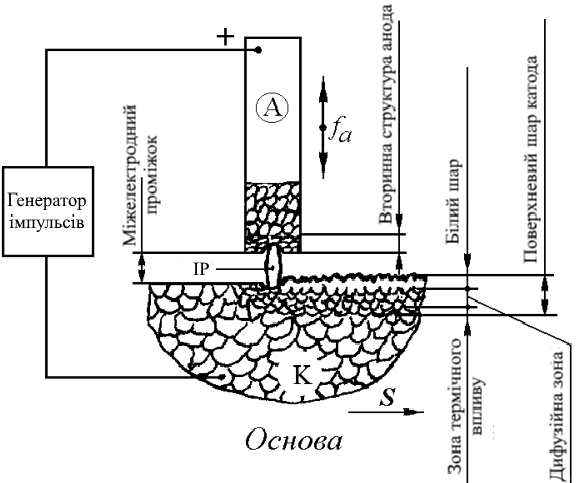
\includegraphics[width=0.7\textwidth]{schema_eil.png}
\fnote{ІР --- іскровий розряд; $f_a$ --- частота вібрацій анода; $S$ --- напрямок подачі деталі; $A$ --- анод; $K$ --- катод}
\caption{Загальна схема процесу ЕІЛ~\cite{ivanov2016}}

\label{fig:schema_eil}
\end{figure}

Внаслідок іскрового розряду потік електронів призводить до локального нагрівання аноду. На поверхні катоду під дією значних теплових навантажень відбуваються мікрометалургійні процеси, які сприяють перемішуванню матеріала катода і анода за взаємодії з компонентами газового середовища, що і призводить до високої адгезії між основою і шаром.~\cite{yarkov2004}

Процес починається зі зближення анода з катодом до відстані за якої починається розряд тривалістю від~\SIrange{e-6}{e-3}{\sec}~\cite{mulin1999}. Після пробою міжелектродного проміжку за рахунок генератора імпульсів на поверхнях електродів з'являються осередки плавлення, випаровування які викликають електричну ерозію матеріалів електродів. Відбувається масоперенос переважно з анода на катод. Після закінчення іскрового розряду і віддалення анода від катода завершується розрив електричного кола. Неперервний процес ЕІЛ відбувається за рахунок періодичної комутації електродів за допомогою спеціального віброприладу.

\subsection{Модель процесу ЕІЛ Б.Р.~Лазаренко і Н.І.~Лазаренко}
\label{subsec:model_lazarenko}

При зближенні електродів напруженість електричного поля між ними збільшується і при певному значенні відбувається пробій. Пучок електронів сфокусовано ударяється об анод --- енергія руху електронів передається поверхневим шарам. Далі матеріал анода локально нагрівається, плавиться і частково випаровується. Капля розплавленого метала відділяється від анода і рухається на катод. В процесі капля встигає нагрітися до високої температури, закипає і вибухає. Коло переривається, дія електричного поля зникає, і частинки летять на катод широким фронтом. Так як перегріті каплі та інші часточки знаходяться в газовому середовищі, то вони можуть ще  й утворювати хімічні сполуки. При досягненні катода розплавлені частки зварюються з ним, частково проникають в його поверхню. Також електрод-анод за цим ударяє поверхню і таким чином відбувається перемішування новоутворених часток. Тобто механічний удар ``проковує'' отримане покриття, збільшуючи тим самим його однорідність та густину. За рахунок того, що процес відбувається в доволі малих об'ємах, можна також вважати, що відбувається так зване надшвидке гартування.~\cite{hitlevich1985}

Ця модель розроблена для ЕІЛ при високих напругах. Якщо напруга не перевищує 200~В, то пробій міжелектродного проміжку відбувається майже при контакті поверхонь електродів через частки середовища --- менше \SI{10}{\mkm}. На початковому етапі такого пробою відбувається ``вибух'', який забезпечує попередню очистку поверхні і подальше формування міжелектродного простору для розвитку плазмового розряду~\cite{miczkevich1977}. Зазначається, що можливий масоперенос від основи до аноду~\cite{lazarenko1965}. В такому разі на поверхні катода утворюється ``лунка'' з піднятими краями. Через це після ЕІЛ поверхня деталі має певну шорсткість.

\subsection{Узагальнена модель процесу ЕІЛ А.Д. Верхотурова}
\label{subsec:model_verkhoturov}

Узагальнена модель процесу ЕІЛ~(рис.~\ref{fig:schema_model-eil}) відрізняється від моделі Лазаренко врахуванням поверхневих явищ на аноді та катоді~\cite{verkhoturov1983}: руйнування електродів в рідкій, паровій та твердій фазі; схоплювання в момент контакту; зміна властивостей поверхонь за рахунок масопереносу та імпульсних навантажень; наявність на катоді в зоні дії іскри мікрованни, яка забезпечує перекристалізацію матеріалів та їх фізико-хімічні взаємодії; обмеження товщини шару за рахунок внутрішніх напружень; дискретний характер формування легованого шару.

Потік електронів призводить до розігріву анода, а магнітне поле створює високий тиск в плазмовому тунелі розряду. В результаті такої дії на поверхні електродів з'являються об'ємні джерела тепла, яке є причиною появи ерозійних лунок на аноді та катоді. В лунці можна виділити три зони(рис.~\ref{fig:schema_model-eil},~б): напружений стан, плавлення та випаровування.

Розмір зон плавлення та випаровування обернено пропорційно залежить від температури плавлення, кипіння та від коефіцієнту теплопровідності електрода. Зона НС виникає за рахунок термічних і термомеханічних напружень в результаті імпульсного нагріву, реактивної дії струменю плазми та її розширення в момент спадання струму в імпульсі. Великі значення розтягуючих напружень на поверхні катода є причиною утворення тріщин та твердофазної ерозії, вклад якої залежить від режиму обробки. Полярний масоперенос (від А до К) відбувається за умови, якщо питома ерозія аноду набагато перевищує суму питомих ерозій утворення тріщин та твердих фаз.~\cite{verkhoturov1988}

\begin{figure}[H]
\centering
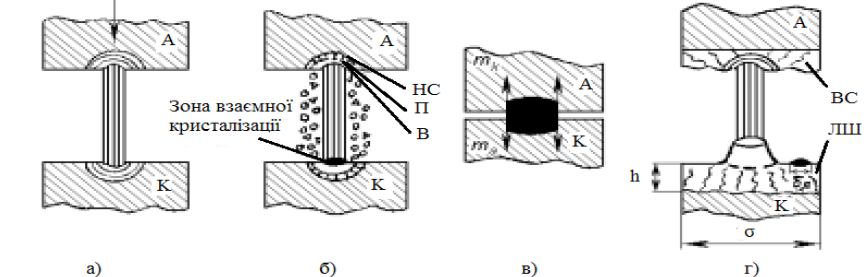
\includegraphics[width=\textwidth]{schema_model-eil.png}
\fnote{а) пробій; б) утворення ерозійних лунок на аноді (А) і катоді (К) з трьома зонами: В~---~випаровування, П~---~плавлення, НС~---~напружений стан; в) момент контакту; г) формування на вторинної структури (ВС) і легованого шару (ЛШ)}
\caption{Узагальнена модель процесу ЕІЛ~\cite{yarkov2004}}
\label{fig:schema_model-eil}
\end{figure}

Багатократна взаємодія іскрових розрядів зумовлює обмеження товщини легованого шару. Основними причинами того є: внутрішні напруження, зменшення термовтоми через багатократне нагрівання та охолодження мікрооб'ємів та утворення ультрадисперсної структури.

Недоліком узагальненої моделі є лише те, що вона не пояснює зв'язок між мікротвердістю електродного матеріалу та легованого шару.

\section{Електродні матеріали для ЕІЛ}

В якості електродного матеріалу для ЕІЛ переважно обирають сплави ВК і ТК~\cite{yarkov2004}. Такий вибір обґрунтований високою твердістю та зносостійкістю даних сплавів. Якщо такий зв'язок властивостей електрода з властивостями отримуваного шару ще можна вважати придатним з деякими обмеженнями, то у випадку нанесення покриттів спеціального призначення (жаростійких, корозійних і т.п.) --- недоцільно.

Часто при виборі електроду звертають увагу на розчинність з матеріалом основи. Бажаною є необмежена розчинність елементів в твердому стані~\cite{yarkov2004}. Для прикладу можна навести такі пари як Fe-Cr, Cu-Ni, Fe-Ni.

Далі розглянуті матеріали, які використовуються в якості анодів для ЕІЛ.

\subsection{Вольфрам та його карбіди}
\label{subsec:tungsten}

Вольфрам здебільшого використовується у виготовленні твердосплавів --- точніше його кабіди --- та для легування різних сплавів, наприклад сталей~\cite{eltit}. WC --- з температурою плавлення \SI{2770}{\degreeCelsius}~\cite{diag1997t1}~(рис.~\ref{fig:phase_diag_C-W} на стор.~\pageref{fig:phase_diag_C-W}) має високу електропровідність, що важливо для процесу ЕІЛ, та використовуються для створення зносостійких абразивів~\cite{daintith2014chemistry}.

Так у випадку легування гальванічних покриттів вольфрамом в~\cite{serebrovsky2012} зазначається, що мікротвердість отриманого покриття може сягати \SI{8.3}{\gpa} в залежності від концентрації легуючого елементу, тобто вольфраму.

\subsection{Хром}
\label{subsec:chrome}

Як електрод для ЕІЛ використовується для підвищення зносо- та жаростійкості, покращення стійкості ріжучого інструмента. Як матеріал основи для легування хромом найчастіше виступають сталь 30, 45, 40Х, У10А ХВГ, ВТ2, Cu~\cite{yarkov2004}. Хром відноситься до перехідних металів, необмежено розчинний з залізом~\cite{diag1997t2}~(рис.~\ref{fig:phase_diag_Cr-Fe} на стор.~\pageref{fig:phase_diag_Cr-Fe}). За рахунок цього при ЕІЛ товщина білого шару може сягати від \SIrange{50}{60}{\mkm}~\cite{sydorenko2013}. Хром не схильний до утворення вторинних структур, які можуть перешкоджати нанесенню матеріалу на оброблювану поверхню.
Випадок з легуванням хромом свідчить про те, що не завжди більшій твердості покриття відповідає більше значення зносостійкості~\cite{hitlevich1985}.

\subsection{Багатошарове нанесення металів з графітом}
\label{subsec:multiplyeil}


Метод електроіскрового легування дає широкі можливості по нанесенню шарів: великий вибір електродів, режими легування, насичуюче середовище. До цього ще можна додати комбінування легованих шарів. Тобто створюють системи з чергуванням твердих та м'яких складових у вигляді як гетерогенних матричних, так і багатошарових структур. Такі системи утворюють двома шляхами: або нанесенням багатошарових покриттів тільки методом ЕІЛ, або комбінування різних методів поверхневих обробок. В першому випадку нанесення в основному проводять для зміцнення(ціллю не є відновлення) ріжучого і штампового інструмента. Наприклад: двошарові покриття твердосплав-графіт, мідь-графіт, хром-графіт або чергування твердосплавів~\cite{yarkov2004}. Також нанесення другого шару проводять для покращення тепловідводу~\cite{yarkov2004}, підвищення жаростійкості~\cite{kadenacy1989}. При цьому важлива узгодженість коефіцієнтів термічного розширення та адгезійна міцність між шарами та з основою~\cite{podchernyaeva2012}.

Багатошаровим нанесенням можна керувати товщиною та шорсткістю легованого шару. Встановлено~\cite{verkhoturova}, що для створення білого шару більшої товщини потрібно наносити шари в такій послідовності: графіт, сплав, а для отримання меншої шорсткості  вигідніше наносити спочатку сплав, а потім графіт. Також проблему товщини шару вирішують електроди, які утворюють необмежені тверді розчини.

\section{Якісна модель ЕІЛ}

Таким чином на основі розглянутих літературних даних можна висловити якісну модель електроіскрового легування з урахуванням підібраних анодних матеріалів у роботі. Також попередні моделі не враховують вплив міжелектродного середовища, яким в даній роботі виступає повітря~(кисень --- $\approx$20\%, азот --- $\approx$70\%), на формування легованого шару.

Опис зближення електродів відповідає моделі Верхотурова, а саме йде мова про наявність надвисоких швидкостей нагрівання, що призводить до локалізованого розплавлення або навіть випаровування матеріалів аноду та катоду.

За цим матеріал аноду переноситься у розплавлену ``мікрованну'' в катоді та перемішується. При цьому частки можуть перебувати в трьох агрегатних станах: рідкому, твердому та газоподібному. Під час переносу матеріалу відбувається іонізація та розкладання молекул газового середовища з утворенням атомарного азоту, який може насичувати розплавлені об'єми обох електродів~\cite{lobachova2012}.

Через малу тривалість термічної дії іскрового розряду не відбувається повне вирівнювання концентрацій в ``мікрованні''. Внаслідок цього в легованому шарі можуть формуватися ділянки, які відрізняються за своїм хімічних складом, які відповідно можуть мати різні коефіцієнти термічного розширення. При надшвидкому охолодженні це призводить до виникнення високих термічних напружень, які додаються до структурних, які в свою чергу зумовлені різким градієнтом температур~\cite{lobachova2012}. Під дією цих напружень виникають дислокації, які переміщюються та в результаті взаємодії між собою утворюють гальмуючі скупчення, які подібні до зон Гін'є~Престона. Після повторних імпульсних нагріваннях концентрація атомів зростає та зони передвиділень перетворюються у дисперсні частинки фаз втілення~\cite{lobachova2012}. Така нерівноважна структура може бути передумовою високої мікротвердості та зносостійкості.

\section{Висновки до розділу~\thechapter}

Отже, щодо ЕІЛ можна зробити висновок, що це метод, який дозволяє проводити ефективний, та керований процес обробки поверхонь металевих матеріалів. Сутність методу також дозволяє використання майже будь-яких електродних матеріалів і внаслідок цього доступний широкий діапазон поліпшення експлуатаційних характеристик поверхонь.

Відповідно до розглянутих матеріалів, можна стверджувати, що використання вольфраму, хрому та вуглецю як анодних матеріалів дає можливість відновити та підвищити зносостійкість повехні певної деталі. Присутність графітового аноду в схемах нанесення спонукає до розгляду таких факторів зміцнення, як формування карбідних складових.

Розглянута якісна модель ЕІЛ, основними етапами якої є:
\begin{itemize}
\item взаємодія атомів матеріалів~(W,Cr) з атомами втілення~(N, C) за екстримальних умов;
\item утворення локальних ділянок на катоді, які відрізняються між собою за хімічним складом та виникнення полів напружень, внаслідок надшвидкого охолодження;
\item дифузія областей передвиділень на скупченнях дислокацій з подальшим перетворенням їх на фази втілення~(карбіди, нітриди, карбонітриди).
\end{itemize}

\chapter{МЕТОДИКА ДОСЛІДЖЕННЯ}

\section{Вихідні матеріали}

В якості матеріалу для формування покриттів ЕІЛ обрана сталь~45, яка має задовільну зварюваність та собівартість.
В табл.~\ref{tab:precursor} наведений хімічний склад даного матеріалу та використованих анодів.

\begin{table}[h!]
\centering
\caption{Хімічний склад вихідних матеріалів для дослідження~\cite{steel45}}
\label{tab:precursor}
\begin{tabular}{|c|c|p{7.9cm}|}
\hline
Матеріал  & Використання у досліді & Хімічний склад, мас.\%\\\hline
Сталь 45&Катод&С~--- 0,42..0,5; Si~--- 0,17..0,37; Mn~--- 0,5..0,8; Ni~--- до~0,25; S~--- до~0,04; P~--- до~0,035; Cr~--- до~0,25; Cu~--- до~0,25; As~--- до~0,08; Fe~--- 97\\\hline
Cr&Анод&Cr~--- 99,9\\\hline
С&Анод&C~--- 99,9\\\hline
W&Анод&W~--- 99,9\\\hline
\end{tabular}
\end{table}


Для отримання зносостійкої поверхні з високою мікротвердістю обрані аноди, які можуть утворювати карбо- та карбонітридні сполуки. Хром в комбінованому шарі слугує ``м’якою підкладкою'', яка може утворювати з залізом твердий розчин з необмеженою розчинністю~(рис.~\ref{fig:phase_diag_Cr-Fe}).

\section{Методика експерименту}

Схема проведення ЕІЛ зображена на рис.~\ref{fig:schema_device}. Зразок (4) надійно закріплюється тримачем, а віброелемент (3) переміщується (вручну) над його поверхнею.

Електроіскрове легування проводилось на установці <<Элитрон-26А>>. На рис.~\ref{fig:elitron_face} зображена панель керування даною установкою. Живлення установки дає мережа 220~В. Тумблером~5 здійснюється корегування струму, що показує амперметр~1, у діапазоні від 0,1~А до 3~А режимами від 1 до 10. Для обох зразків режим становив 2~А і процес відбувався на повітрі за кімнатної температури.


\begin{figure}[H]
\centering
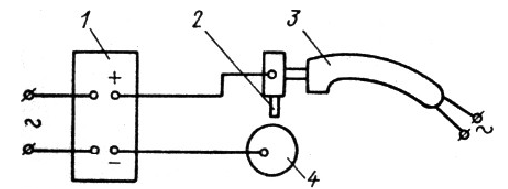
\includegraphics[width=0.5\textwidth]{schema_device.png}
\fnote{1 – генератор імпульсів; 2 --- легуючий електрод; 3 --- електромагнітний віброелемент; 4 --- зразок (катод)}
\caption{Схема установки для ЕІЛ~\cite{ivanov2016}}
\label{fig:schema_device}
\end{figure}


\begin{figure}[H]
\centering
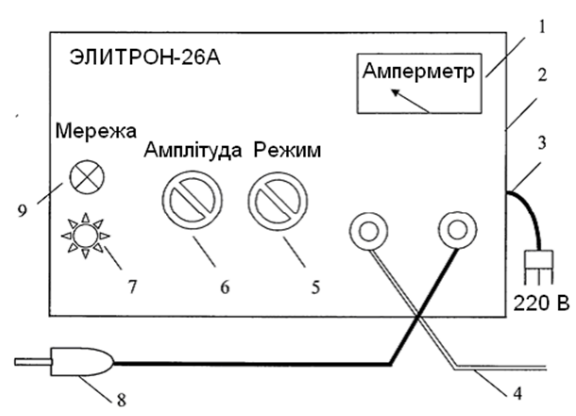
\includegraphics[width=0.55\textwidth]{elitron_face.png}
\fnote{1~---~амперметр; 2~---~генератор; 3~---~кабель живлення; 4~---~з’єднувальний кабель (на катод); 5~---~тумблер ступінчастого регулювання режиму; 6~---~тумблер регулювання амплітуди коливання аноду; 7~---~вмикач живлення установки; 8~---~віброелемент (на анод); 9~---~сигнальна лампочка}
\caption{Панель керування установки <<Элитрон-26А>>~\cite{ivanov2016}}
\label{fig:elitron_face}
\end{figure}

Для досягнення мети дослідження було проведено ЕІЛ чотирьох зразків за схемами Cr-W-C, W-C-Cr, W-Cr-C, C-Cr-W по 3 хвилини на кожен етап нанесення аноду.

\section{Методика дослідження}

В роботі використана комплексна методика дослідження, яка включає гравіметричний метод, мікроструктурний та мікродюрометричний аналіз, випробування на зносостійкість. Такий комплекс забезпечує вивчення процесів та явищ згідно з метою роботи та задовільну точність вимірювання.

\subsection{Гравіметричний метод}
\label{subsec:method_gravi}

Метод полягає у вимірюванні маси зразків та електродів до легування та під час процесу з кроком в 1 хвилину. Для вимірювання використовувались лабораторні електронні ваги AXIS~AD50 з точністю 0,0005~г.

Для оцінки процесу формування легованого шару визначають такі характеристики як ерозію аноду~$\Delta m^a$ та приріст маси катоду~$\Delta m^k$. Ці значення розраховуються як різниця маси в момент часу $t_{n}$ та за попередній вимір $t_{n-1}$:
\begin{equation}
\Delta m_t  = m(t_n)-m(t_{n-1}).
\label{eq:deltam}
\end{equation}
Оскільки сума даних значень дорівнює різниці маси за останній вимір та початкової маси, то сумарна ерозія $\Delta$ за час $t$ розраховується за формулою:
\begin{equation}
\Delta_t = m(t)-m(t_0),
\label{eq:erosion}
\end{equation}
\begin{eqitemize}
\item[де] $m(t_0)$ --- початкова маса перед обробкою;
\item $m(t)$ --- маса після обробки за час $t$.
\end{eqitemize}

Аналогічно розраховується і приріст ваги катоду $\Delta_t^k$  але з протилежним значенням. Питомі значення цих величин відображають масоперенос на одиницю пройденого заряду. Таким чином питома ерозія $G$ за  розраховується за формулою:
\begin{equation}
G = \frac{\Delta m_t}{I \cdot \Delta t},
\label{eq:specific_erosion}
\end{equation}
\begin{eqitemize}
\item[де] $\Delta m_t$ --- ерозія аноду або приріст ваги катоду;
\item $I$ --- сила струму;
\item $\Delta t$ --- час, за який відбувалася ерозія $\Delta m_t$.
\end{eqitemize}

Коефіцієнт масопереносу розраховується з відношення:
\begin{equation}
K = \frac{G^a}{G^k},
\label{eq:masstransfer_coef}
\end{equation}
\begin{eqitemize}
\item[де] $G^a$ --- питома ерозія аноду;
\item $G^k$ --- питомий приріст катоду.
\end{eqitemize}

Отже для отримання усередненого значення масопереносу маємо за час~$t$:
\begin{equation}
\bar{K}_t = \frac{\sum_{i=0}^{i=n} K_i}{n},
\label{eq:average_masstransfer_coef}
\end{equation}
\begin{eqitemize}
\item[де] $n$ --- кількість вимірів за час $t$.
\end{eqitemize}

До часових характеристик відносяться такі якісні величини: $t_x$ --- поріг крихкого руйнування нанесеного шару --- час, якому відповідає максимальне значення $\Delta_t^k$ (момент першого від'ємного приросту $\Delta m$); $t_{cr}$ --- критичний поріг руйнування поверхневого шару --- час, якому відповідає нульове значення $\Delta_t^k$, при $t \neq 0$.

Отже згідно з~\cite{mulin1999} можемо розрахувати ефективність процесу утворення зміненого поверхневого шару:
\begin{equation}
\Upsilon_{t_x} = \bar{K}_{t_x} \cdot t_x \cdot \sum_{t=0}^{t_x} \Delta m_t^k;
\label{eq:effectiveness_coef_x}
\end{equation}
та ефективність процесу утворення зміненої поверхні:
\begin{equation}
\Upsilon_{t_{cr}} = \bar{K}_{t_{cr}} \cdot t_{cr} \cdot \sum_{t=0}^{t_{cr}} \Delta m_t^k.
\label{eq:effectiveness_coef_cr}
\end{equation}

Останні дві характеристики дають можливість порівнювати матеріали елетродів за їх впливом на формування шару~\cite{yarkov2004}.

\subsection{Мікроструктурний аналіз}
\label{subsec:microstructure_analysis}

Для дослідження за допомогою оптичного мікроскопу зі зразків виготовляли металографічні поперечні мікрошліфи. Підготовка шліфів проводилась таким чином. Зразки затискаються у струбцині і шліфуються на абразивному колі. Далі проводиться поетапне шліфування на корундових паперах зі зміною напрямку шліфування перед переходом на папір з меншим зерном. Після отримання поверхні з задовільною шорсткістю без подряпин проводять полірування на фетрі з використанням оксиду хрому, а потім на воді. Отримані шліфи протравлені \SI{5}{\percent} розчином азотної кислоти в етиловому спирті.

Дослідження та фотографування мікроструктури проводилось на металографічному мікроскопі МІМ-10 при збільшенні у 400 разів.

\subsection{Мікродюрометричний аналіз}
\label{subsec:microhardness_analysis}

Мікротвердість зразків вимірювали на приладі ПМТ-3М. Визначення мікротвердості полягає у вдавлюванні індентора при навантаженні \SI{0.02}{\kilog} протягом 10~секунд. Індентор --- алмазна пірамідка з квадратною основою і кутом при вершині 136\degree. За допомогою об’єкт-мікрометра визначають довжини діагоналей ромбу декілька разів. По табличним даним приладу визначається мікротвердість в ГПа за середнім значенням діагоналей видавленого ромба.

\subsection{Випробування на зносостійкість}
\label{subsec:wear_resisting_analysis}

Випробування на зносостійкість проводилась на установці, схема якої зображена на рис.~\ref{fig:schema_original_set}, в умовах сухого тертя за схемою ``площина по площині'' протягом 2~годин.

\begin{figure}[H]
\centering
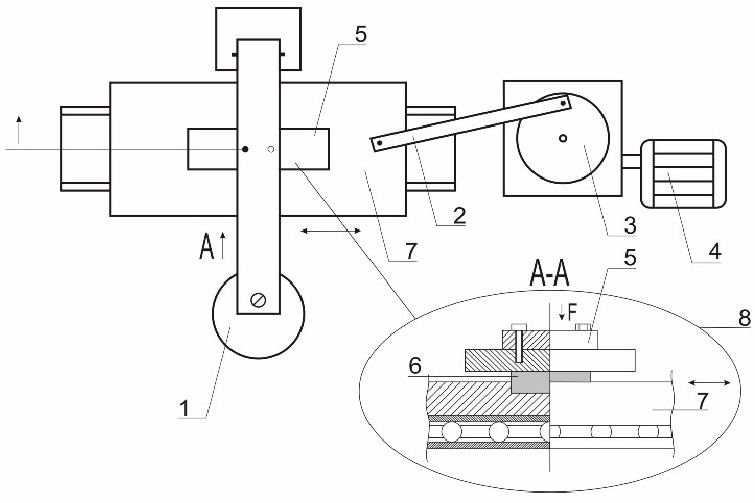
\includegraphics[width=0.5\textwidth]{schema_original_set.png}
\fnote{1 --- навантаження; 2 --- шатун; 3 --- колінчата передача; 4 --- електродвигун; 5 --- контртіло; 6 --- зразок; 7 --- станина; 8 --- загальна схема тертя}
\caption{Схема оригінальної установки на тертя без мастила}
\label{fig:schema_original_set}
\end{figure}
Обертання від електродвигуна постійного струму передається на шатун. Рухома платформа здійснює зворотно-поступальний рух по коліям за допомогою шатуна, прикріпленого до обертальної частини редуктора. На рухомій платформі розміщено досліджуваний зразок, який контактує з контртілом (сталь Р6М5), закріпленим на важелі, під час дії навантаження (гиря) \SI{3}{\kilog}.

Величина зношування вимірювалася ваговим методом. Зразок через кожні 30~хв зважується на вагах AXIS~AD50~(стор.~\pageref{subsec:method_gravi}). За втратою маси обчислюється показник інтенсивності зношування:
\begin{equation}
I = \frac{\Delta m}{S},
\label{eq:wear_intensity_coef}
\end{equation}
\begin{eqitemize}
\item[де] $\Delta m$ --- втрата маси, кг;
\item $S$ --- площа поверхні тертя зразка, $\text{м}^2$.
\end{eqitemize}

\subsection{Рентгеноструктурний аналіз}
\label{subsec:rentgen}

Рентгеноструктурний аналіз --- це ідентифікація кристалічних фаз і визначення їх відносних концентрацій у сумішах на основі аналізу дифракційної картини, яку реєстрованої від досліджуваних зразків~\cite{horelik1994}.

Аналіз полягає у проведенні порівняння експериментальних значень міжплощинних відстаней і відносних значень інтенсивності з довідковими даними~(еталонні рентгенограми). Таким чином можна визначити склад неметалевих включень в металах та ідентифікувати окремі фази гетерогенної системи.

Рентгеноструктурний аналіз зразків проводився на дифрактометрі Rigaku~Ultima~4. Зйомки велись на мідному монохроматизованому випромінені при напрузі 30~кВ та струмі~30 мА.

Ідентифікація фаз проводилась за картотекою ASTM шляхом порівняння експериментальних даних та даних з міжплощинних відстаней~$(d)$ та інтенсивності ліній, які були отримані при зйомці рентгенограм. При кількості збігів менше трьох рефлексів визначена фаза вважалася відсутньою.

Визначення міжплощинних відстаней проводилося за формулою Вульфа-Бреггів:
\begin{equation}
2d sin\theta=n\lambda,
\label{eq:wulfbregg}
\end{equation}
\begin{eqitemize}
\item[де] $d$ --- міжплощинна відстань;
\item $\theta$ --- бреггівський кут.
\end{eqitemize}

Період гратки матеріалу розраховується за формулою:
\begin{equation}
a = \frac{\lambda}{2sin\theta} \sqrt{H^2+K^2+L^2},
\label{eq:lattice_period}
\end{equation}
\begin{eqitemize}
\item[де] $H, K, L$ --- індекси площин відбиття;
\item $\lambda$ --- довжина хвилі.
\end{eqitemize}

Рентгенограми, які отримані від багатофазних систем є результатом накладання дифракційних ліній від окремих фаз. Фаза, вміст якої відносно малий, може бути представлена на рентгенограмі лише невеликою кількістю найбільш інтенсивних ліній.

\subsection{Комп'ютерні методи}
\label{subsec:label}

Зручно організований обчислювальний процес --- один з найважливіших етапів проведення прикладних досліджень або виконання інженерних розрахунків. Зараз комп'ютерні можливості дозволяють виконувати складні автоматизовані алгоритми з гнучким налаштуванням та високою швидкістю виконання. Також використання автоматизованих алгоритмів в роботі допомагає виключати помилки людського чиннику, особливо ті, які відбуваються під час ручного виконання однотипних операцій --- явище ``блукаючого розуму''~\cite{maillet2017}.

Отже для реалізації обчислювального середовища для вирішення матеріалознавчих задач необхідне і достатнє використання таких пакунків на базі мови програмування Python:
\begin{itemize}
\item NumPy --- пакет для високошвидкісної роботи з масивами даних;
\item Pandas --- зручний засіб для початкової обробки даних, завантаження їх в обчислювальне середовище, вибору значень за певними критеріями, роботи з пропущеними даними, експорту даних в вигляді таблиць в середовище \LaTeX;
\item Matplotlib --- пакет для візуалізації результатів обчислень, дозволяє здійснювати гнучке налаштування графіків, впроваджувати формульні написи на графіках з використанням середовища \LaTeX;
\item Scikit-image --- пакет для обробки зображень. \label{text:scikit-image}
\end{itemize}

Таким чином для реалізації обробки результатів розроблені виконуючі программи для гравіметричного, мікроструктурного та мікродюрометричного аналізів. Лістинги розроблених скриптів наведені в додатку~\ref{app:listings}.

\section{Висновки до розділу~\thechapter}

Для досягнення поставленої задачі переддипломної практики розроблений та проведений процес ЕІЛ сплаву сталь~45 анодами Cr, C, W без захисного середовища на повітрі за схемами Cr-W-C, W-C-Cr, W-Cr-C, C-Cr-W.

Обґрунтовано вибір вихідних матеріалів та легувальних електродів для дослідження.

Визначена комплексна методика дослідження, яка дає можливість отримати достовірні результати вимірювання, які дозволяють детально проаналізувати отримані експериментальні дані та дати їм об’єктивну оцінку.


\chapter{РЕЗУЛЬТАТИ ТА ЇХ ОБГОВОРЕННЯ}

\section{Формування покриття на сталі~45 під час ЕІЛ за схемою Cr-W-C}

Дослідження зразка сталі~45, після ЕІЛ за схемою легування Cr-W-C, показало, що товщина легованого шару знаходиться в межах від \SIrange{15}{35}{\mkm}. На деяких ділянках спостерігається розтріскування~(рис.~\ref{fig:adapt_microstr_Cr-W-C}). Під легованим шаром роташовується тонка смуга зони термічного впливу з дрібними зернами.

\begin{figure}[H]
\centering 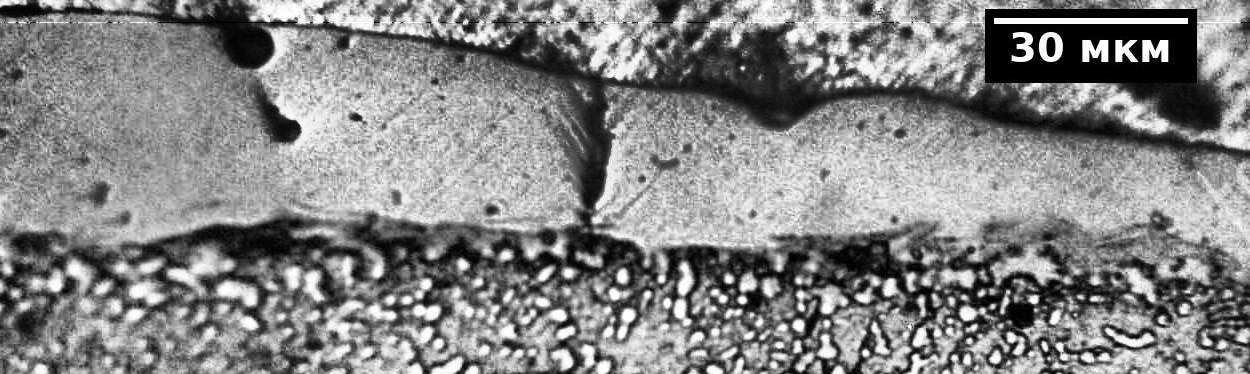
\includegraphics[width=\textwidth]{adapt_gray_microstr_Cr-W-C.jpg}
\caption{Мікроструктура поверхні сталь~45 після ЕІЛ за схемою Cr-W-C}
\label{fig:adapt_microstr_Cr-W-C}
\end{figure}

За результатами гравіметричного аналізу були кінетичні криві масопереносу~(сумарного приросту маси катоду $\sum \Delta m_k$ та сумарної ерозії анодів $\sum \Delta m_a$), які наведені на рис.~\ref{fig:plt_gravi_Cr-W-C}.

\begin{figure}[H]
\centering  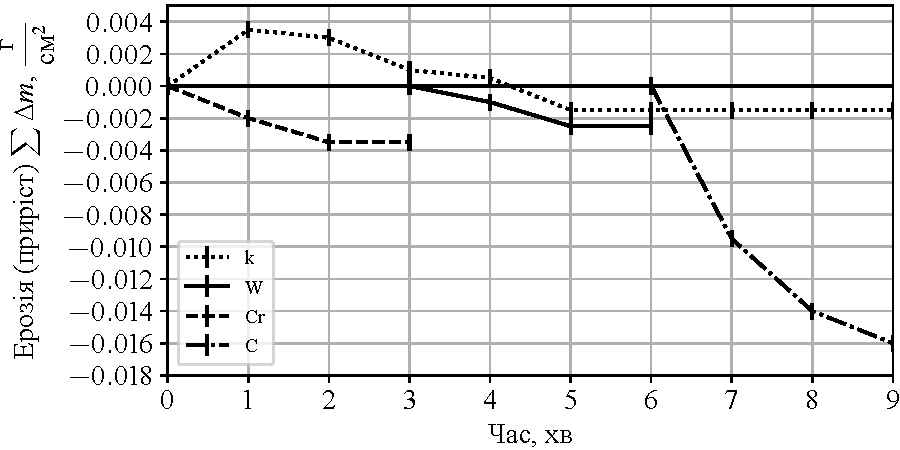
\includegraphics[]{plt_gravi_Cr-W-C.pdf}
\caption{Кінетика масоперенесення під час ЕІЛ за схемою Cr-W-C}
\label{fig:plt_gravi_Cr-W-C}
\end{figure}

На першому етапі легування~(нанесення хрому) спостерігається додатній приріст маси катоду. Критичний поріг руйнування поверхневого шару знаходиться на 4-й хвилині процесу, тобто  на першій хвилині нанесення вольфраму.

Третій етап, а саме легування графітом не вніс зміни на катод. Ерозія анодних матеріалів відбувається під час кожної стадії ЕІЛ. Слід зазначити, що сумарна ерозія W-аноду є найменшою з усіх обраних матеріалів через його тугоплавкість. Найбільшу ерозію має графітовий електрод, оскільки для нього характерний великий опір~(від \SIrange{3d-5}{60d-5}{\mkomm}~\cite{web:resistivity}). Розрахована ефективність за формулами \eqref{eq:effectiveness_coef_x} і \eqref{eq:effectiveness_coef_cr} становить відповідно 2 та 4,5.



Фазовий аналіз показав, що в покритті присутні такі фази карбідів $\epsilon$-Fe\textsubscript{3}C та Cr\textsubscript{3}C\textsubscript{2}, а також графіт у незв'язаному стані~(рис.~\ref{tab:peaks_Cr-W-C}, табл.~\ref{fig:peaks_Cr-W-C}).
\begin{figure}[H]
\centering
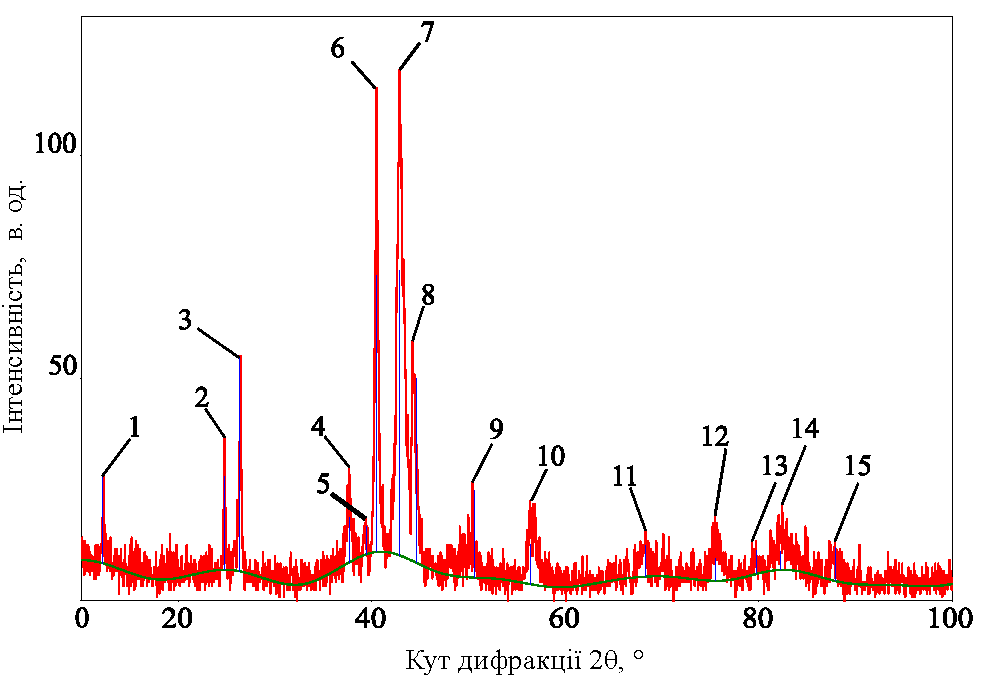
\includegraphics[width=\textwidth]{rigaku_peaks_Cr-W-C.ps}
\caption{Дифрактограма покриття Cr-W-C після ЕІЛ сталі~45}
\label{fig:peaks_Cr-W-C}
\end{figure}

Розраховані періоди кристалічних ґраток кожної фази, параметри субструктури (області когерентного розсіювання та мікровикривлення ґратки) наведені в табл.~\ref{tab:structure_Cr-W-C}.

\begin{table}[H]
\centering
\caption{Фазовий склад покриття Cr-W-C після ЕІЛ сталі~45}
\label{tab:peaks_Cr-W-C}
\begin{tabular}{|l|c|c|l|c|}
  \hline
  \multicolumn{1}{|c|}{№} & \multicolumn{1}{c|}{Кут дифракції 2$\theta$, \degree} & \multicolumn{1}{c|}{Міжплощинна відстань d, \AA} &  \multicolumn{1}{c|}{Фаза} & \multicolumn{1}{c|}{HKL} \\ \hline
  1 & 12 & 7,2516 & графіт & 004 \\ \hline
  2 & 25 & 3,5843 & графіт & 008 \\ \hline
  3 & 26 & 3,3850 & графіт & 002 \\ \hline
  4 & 38 & 2,3846 & $\epsilon$-Fe\textsubscript{3}C & 110 \\ \hline
  5 & 39 & 2,2808 & Cr\textsubscript{3}C\textsubscript{2} & 112 \\ \hline
  6 & 41 & 2,2230 & Cr\textsubscript{3}C\textsubscript{2} & 203 \\ \hline
  7 & 43 & 2,1052 & Cr\textsubscript{3}C\textsubscript{2} & 113 \\ \hline
  8 & 45 & 2,0277 & графіт & 101 \\ \hline
  9 & 51 & 1,8021 & Cr\textsubscript{3}C\textsubscript{2} & 301 \\ \hline
  10 & 56 & 1,6284 & $\epsilon$-Fe\textsubscript{3}C & 112 \\ \hline
  11 & 68 & 1,3717 & $\epsilon$-Fe\textsubscript{3}C & 300 \\ \hline
  12 & 76 & 1,2583 & графіт & 110 \\ \hline
  13 & 80 & 1,2012 & $\epsilon$-Fe\textsubscript{3}C & 220 \\ \hline
  14 & 82 & 1,1714 & $\epsilon$-Fe\textsubscript{3}C & 302 \\ \hline
  15 & 88 & 1,1096 & графіт & 006 \\ \hline

  \end{tabular}
\end{table}

\begin{table}[H]
\centering
\caption{Параметри структури покриття Cr-W-C}
\label{tab:structure_Cr-W-C}
\begin{tabular}{|l|r|r|r|c|r|}
\hline
\multicolumn{1}{|c|}{\multirow{2}{*}{Фаза}} & \multicolumn{3}{c|}{Періоди ґратки, \AA} & \multicolumn{1}{c|}{\multirow{2}{*}{Розміри ОКР, \AA}} & \multicolumn{1}{c|}{\multirow{2}{*}{Мікронапруження  $\frac{\Delta d}{d}$, \%}} \\ \cline{2-4}
\multicolumn{1}{|c|}{} & \multicolumn{1}{c|}{a} & \multicolumn{1}{c|}{b} & \multicolumn{1}{c|}{c} & \multicolumn{1}{c|}{} & \multicolumn{1}{c|}{} \\ \hline

$\epsilon$-Fe\textsubscript{3}C & 4,77 & -- & 4,44 & 83 & 0 \\ \hline
Cr\textsubscript{3}C\textsubscript{2} & 5,55 & 2,81 & 11,44 & 9 & 0,00312 \\ \hline
графіт & 2,46 & 4,15 & 28,67 & 90 & 0,342 \\ \hline
\end{tabular}
\end{table}

На рис.~\ref{fig:plt_hard_Cr-W-C} за даними мікродюрометричного аналізу поперечного мікрошліфа зразка сталі~45 з нанесеним шаром Cr-W-C побудована залежність мікротвердості від глибини залягання. Виміри проводилися до глибини \SI{50}{\mkm}. Кожне виміряне значення є середнім арифметичним трьох вимірів на відповідній глибині.

Таким чином виявлено, що при легуванні з використанням схеми Cr-W-C на повітрі найбільше значення мікротвердості становить \SI{11.5}{\gpa}, що приблизно у 5~разів більше за мікротвердість cталі~45~(\SI{2.4}{\gpa}~\cite{steel45}).

За результатами випробування на зносостійкість в умовах сухого тертя за схемою ``площина по площині'' протягом 2~годин гравіметричним методом побудована часова залежність інтенсивності зношування для зразку Cr-W-C~(рис.~\ref{fig:plt_wear_Cr-W-C}).

\begin{figure}[H]
\centering
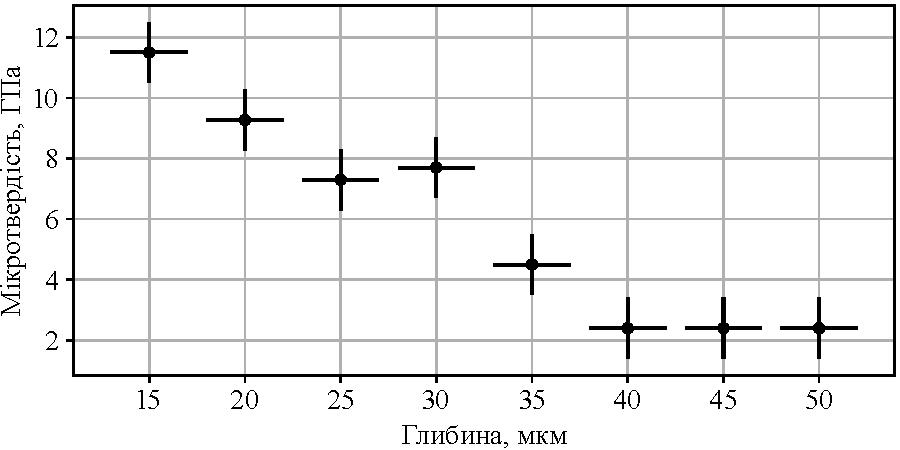
\includegraphics[]{plt_hard_Cr-W-C.pdf}
\caption{Мікротвердість повехневої зони сталі~45 після ЕІЛ за схемою Cr-W-C}
\label{fig:plt_hard_Cr-W-C}
\end{figure}

\begin{figure}[H]
\centering
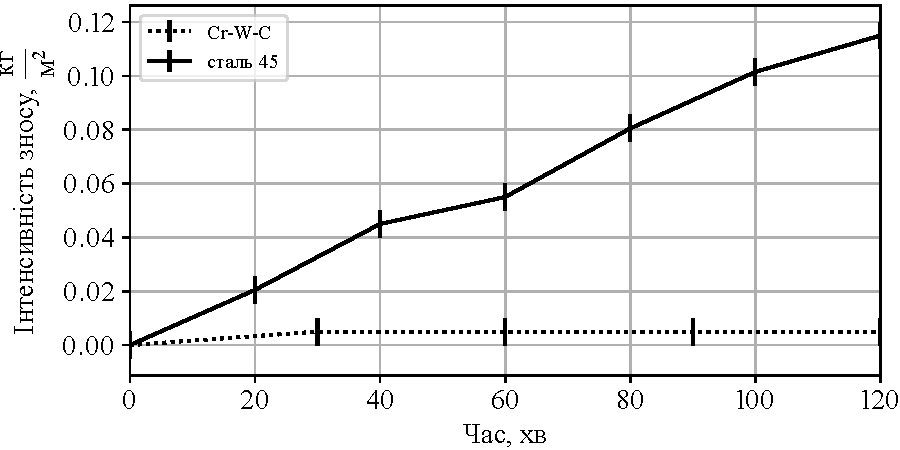
\includegraphics[]{plt_wear_Cr-W-C.pdf}
\caption{Залежність інтенсивності зносу від часу для зразку Cr-W-C}
\label{fig:plt_wear_Cr-W-C}
\end{figure}

З 30 хвилини зміни показника інтенсивності не спостерігається, виникає так звана ``поличка зносу'', яка свідчить про те, що дана поверхня зносостійка. Інтенсивність зносу зразку, який легований за даною схемою у 23~рази менша за інтесивність зносу сталі~45 без обробки. Таке збільшення може бути спричинене формуванням в легованому шарі вільного графіту.

\section{Формування покриття на сталі~45 під час ЕІЛ за схемою W-Cr-C}

В результаті дослідження зразка зі сталі~45, після ЕІЛ з використанням схеми легування W-Cr-C, було встановлено, що товщина легованого шару у середньому становить від 15~мкм до 30~мкм. Покриття має пори та тріщини~(рис.~\ref{fig:adapt_microstr_W-Cr-C}).

Під легованим шаром на мікроструктурі добре спостерігається зона термічного впливу, що може свідчити про високу адгезію з матеріалом основи.

\begin{figure}[H]
\centering 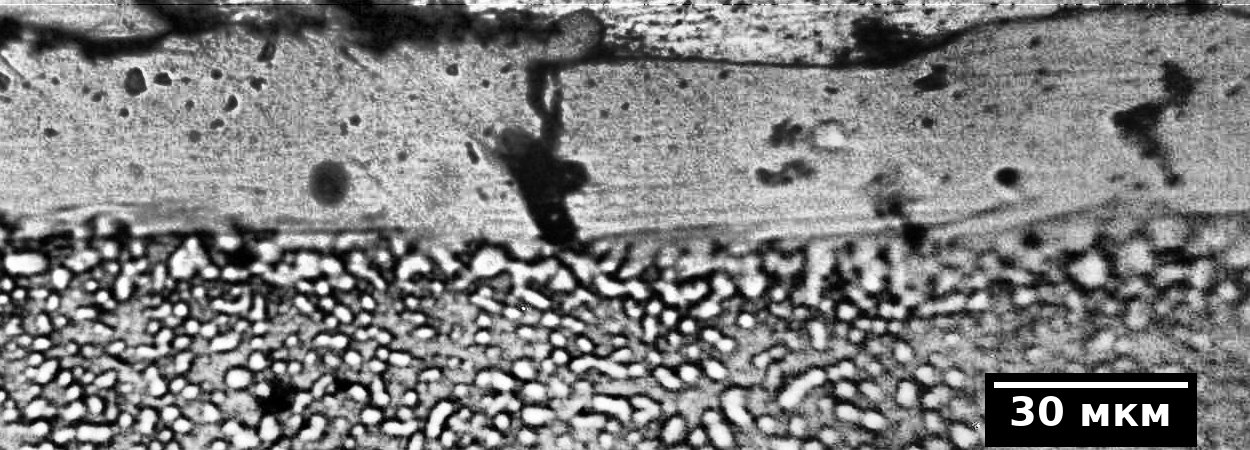
\includegraphics[width=\textwidth]{adapt_gray_microstr_W-Cr-C.jpg}
\caption{Мікроструктура поверхні сталь~45 після ЕІЛ за схемою W-Cr-C}
\label{fig:adapt_microstr_W-Cr-C}
\end{figure}

За результатами гравіметричного аналізу була вивчена кінетика масопереносу~(рис.~\ref{fig:plt_gravi_W-Cr-C}).

\begin{figure}[H]
\centering 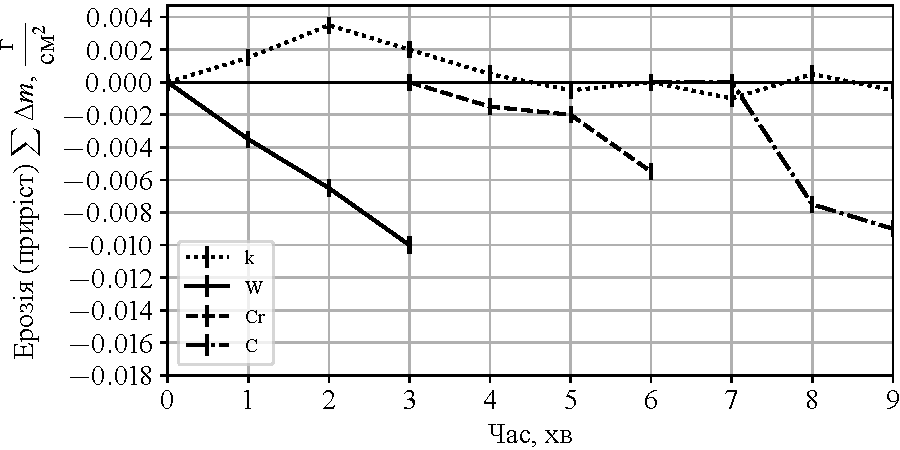
\includegraphics[]{plt_gravi_W-Cr-C.pdf}
\caption{Кінетика масоперенесення під час ЕІЛ за схемою W-Cr-C}
\label{fig:plt_gravi_W-Cr-C}
\end{figure}

Перший етап легування вольфрамом дав додатній приріст маси катоду. Критичний поріг руйнування відповідає процесу, коли крива $\sum \Delta m_k$ перетинає вісь абсцис ---  5-ій хвилині. Другий етап легування хромом спричинив ерозію катоду. Другий та третій етап легування майже не вніс змін в приріст маси катоду.

В результаті фазового аналізу отримана дифрактограма поверхні W-Cr-C~(рис.~\ref{fig:peaks_W-Cr-C}).  Внаслідок проведення розшифровки~(табл.~\ref{tab:peaks_W-Cr-C}) даної дифрактограми в зразку були знайдені карбідні фази WC, W\textsubscript{2}C та Fe\textsubscript{3}C.


\begin{figure}[H]
\centering
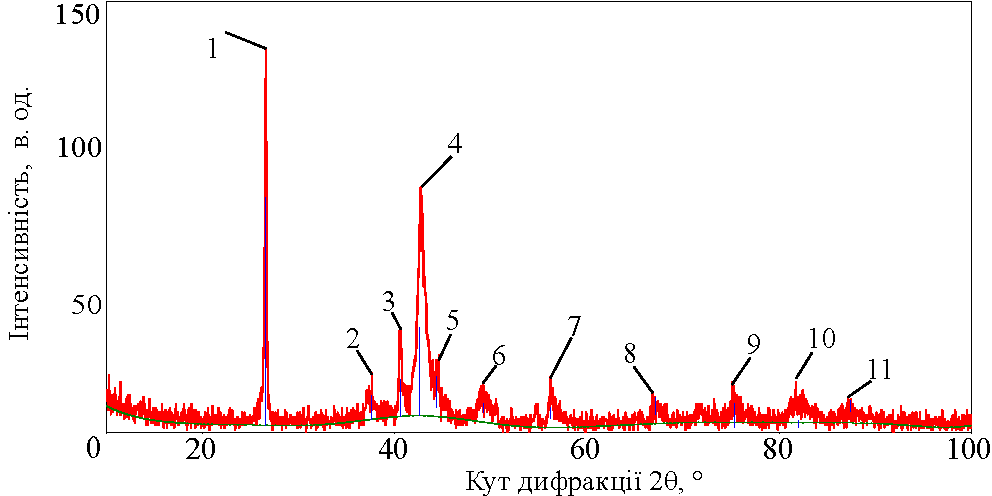
\includegraphics[width=\textwidth]{rigaku_peaks_W-Cr-C.ps}
\caption{Дифрактограма покриття Cr-W-C після ЕІЛ сталі~45}
\label{fig:peaks_W-Cr-C}
\end{figure}

\begin{table}[H]
\centering
\caption{Фазовий склад покриття W-Cr-C після ЕІЛ сталі~45}
\label{tab:peaks_W-Cr-C}
\begin{tabular}{|l|c|c|l|c|}
  \hline
  \multicolumn{1}{|c|}{№} & \multicolumn{1}{c|}{Кут дифракції 2$\theta$, \degree} & \multicolumn{1}{c|}{Міжплощинна відстань d, \AA} &  \multicolumn{1}{c|}{Фаза} & \multicolumn{1}{c|}{HKL} \\ \hline
  1 & 27 & 3,3483 & Fe\textsubscript{3}C & 101 \\ \hline
  2 & 38 & 2,3905 & W\textsubscript{2}C & 002 \\ \hline
  3 & 41 & 2,2193 & Fe\textsubscript{3}C & 201 \\ \hline
  4 & 43 & 2,1233 & W\textsubscript{2}C & 211 \\ \hline
  5 & 44 & 2,0414 & Fe\textsubscript{3}C & 031 \\ \hline
  6 & 49 & 1,8491 & WC & 101 \\ \hline
  7 & 56 & 1,6366 & Fe\textsubscript{3}C & 212 \\ \hline
  8 & 67 & 1,3943 & WC & 002 \\ \hline
  9 & 75 & 1,2598 & W\textsubscript{2}C & 112 \\ \hline
  10 & 82 & 1,1755 & WC & 201 \\ \hline
  11 & 87 & 1,1144 & Fe\textsubscript{3}C & 303 \\ \hline
  \end{tabular}
\end{table}

Розраховані періоди кристалічних ґраток кожної фази, параметри субструктури (області когерентного розсіювання та мікровикривлення ґратки) наведені в табл.~\ref{tab:structure_W-Cr-C}.

\begin{table}[H]
\centering
\caption{Параметри структури покриття W-Cr-C}
\label{tab:structure_W-Cr-C}
\begin{tabular}{|l|r|r|r|c|r|}
\hline
\multicolumn{1}{|c|}{\multirow{2}{*}{Фаза}} & \multicolumn{3}{c|}{Періоди ґратки, \AA} & \multicolumn{1}{c|}{\multirow{2}{*}{Розміри ОКР, \AA}} & \multicolumn{1}{c|}{\multirow{2}{*}{Мікронапруження  $\frac{\Delta d}{d}$, \%}} \\ \cline{2-4}
\multicolumn{1}{|c|}{} & \multicolumn{1}{c|}{a} & \multicolumn{1}{c|}{b} & \multicolumn{1}{c|}{c} & \multicolumn{1}{c|}{} & \multicolumn{1}{c|}{} \\ \hline

WC & 2,9547 & 2,9547 & 2,7826 & 65,16 & 0,0 \\ \hline
W\textsubscript{2}C & 2,9924 & 2,9924 & 4,7651 & 8,7 & 0,0031 \\ \hline
Fe\textsubscript{3}C & 5,1196 & 6,7278 & 4,441 & 50,97 & 0,695 \\ \hline

\end{tabular}
\end{table}

За даними мікродюрометричного аналізу (рис.~\ref{fig:plt_hard_W-Cr-C}) виявлено, що при легуванні з використанням схеми W-Cr-C на повітрі найбільше значення мікротвердості становить \SI{12.8}{\gpa}, що приблизно у 6~разів більше за мікротвердість cталі~45. Це можна пояснити формуванням в легованому шарі карбідів вольфраму.

\begin{figure}[H]
\centering
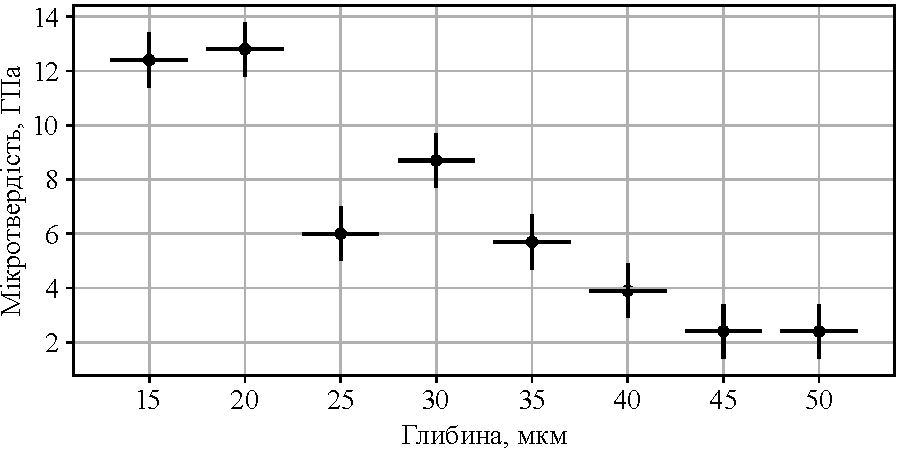
\includegraphics[]{plt_hard_W-Cr-C.pdf}
\caption{Мікротвердість повехневої зони сталі~45 після ЕІЛ за схемою W-Cr-C}
\label{fig:plt_hard_W-Cr-C}
\end{figure}

Випробування на зносостійкість було проведено в умовах сухого тертя за схемою ``площина по площині'' протягом 2~годин. В результаті побудована часова залежність інтенсивності зношування для зразку W-Cr-C~(рис.~\ref{fig:plt_wear_W-Cr-C}). При порівнянні інтенсивностей зношування для легованого зразка та зразка без обробки виявлено, що інтенсивність обробленого зразка у 7,7 разів більша за варіант без сформованого покриття.

\begin{figure}[H]
\centering
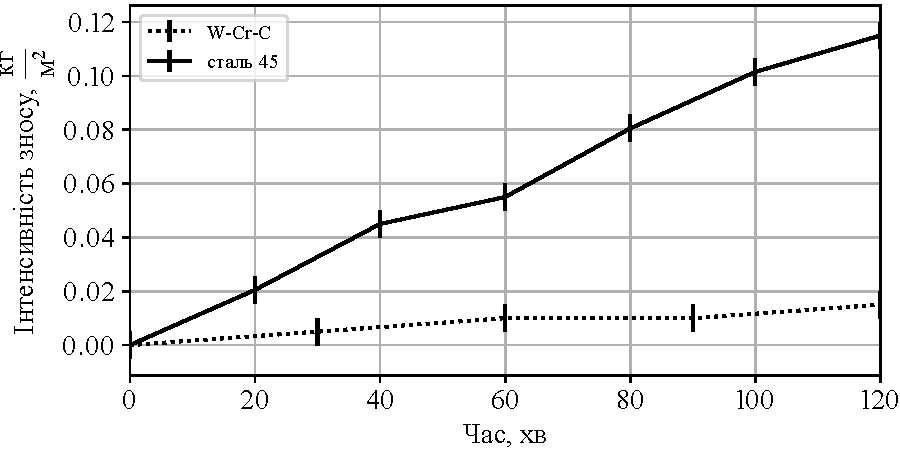
\includegraphics[]{plt_wear_W-Cr-C.pdf}
\caption{Залежність інтенсивності зносу від часу для зразку W-Cr-C}
\label{fig:plt_wear_W-Cr-C}
\end{figure}

Для даного зразку з обробкою поверхні за схемою W-Cr-C ``поличка зносостійкості'' виявляється починаючи з 60-ої хвилини випробування.

\section{Формування покриття на сталі~45 під час ЕІЛ за схемою W-C-Cr}

В результаті дослідження зразка зі сталі~45, з обробкою ЕІЛ з використанням схеми легування, було встановлено, що товщина легованого шару, одержаного на поверхні сталі~45 після ЕІЛ за схемою W-C-Cr становить від 15~мкм до 25~мкм. Під покриттям спостерігається тонкий шар зони термічного впливу, що може свідчити про міцність зчеплення з матеріалом основи~(рис.~\ref{fig:adapt_microstr_W-C-Cr}).

\enlargethispage{1\baselineskip}
\begin{figure}[H]
\centering
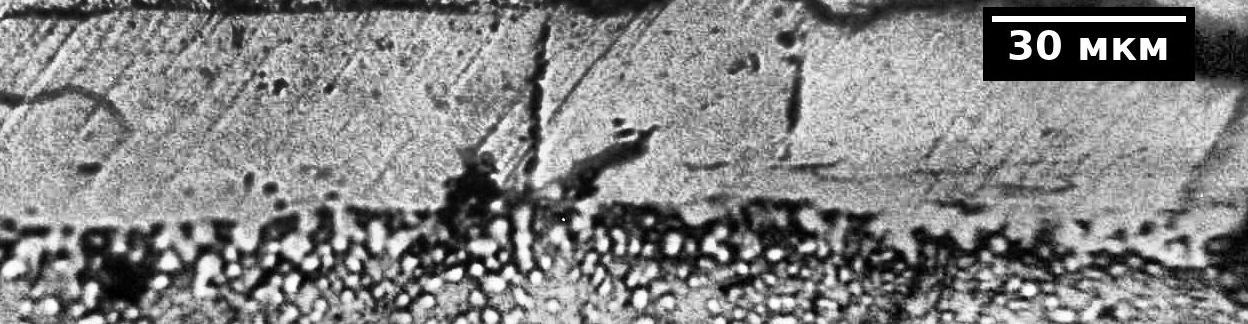
\includegraphics[width=\textwidth]{adapt_gray_microstr_W-C-Cr.jpg}
\caption{Мікроструктура поверхні сталі~45 після ЕІЛ за схемою W-C-Cr}
\label{fig:adapt_microstr_W-C-Cr}
\end{figure}

Кінетика масопереносу в процесі ЕІЛ наведена на рис.~\ref{fig:plt_gravi_W-C-Cr}.

\begin{figure}[H]
\centering 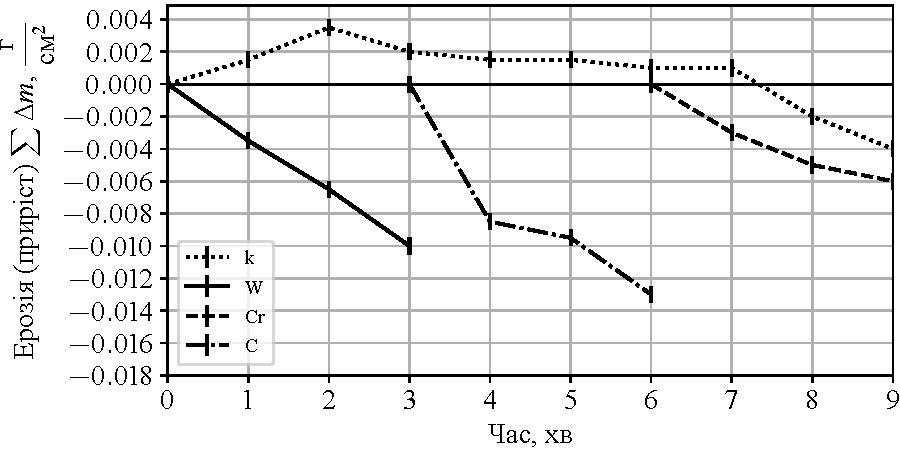
\includegraphics[]{plt_gravi_W-C-Cr.pdf}
\caption{Кінетика масоперенесення під час ЕІЛ за схемою W-C-Cr}
\label{fig:plt_gravi_W-C-Cr}
\end{figure}

На першій стадії етап легування вольфрамом зафіксовано додатній приріст маси катоду. На другій та третій стадії крива~$\sum \Delta m_k$ спадає. Розрахований критичний поріг руйнування маємо на 8-ій хвилині.

Для проведення фазового аналізу була отримана дифрактограма поверхні W-C-Cr~(рис.~\ref{fig:peaks_W-C-Cr}).

\begin{figure}[H]
\centering
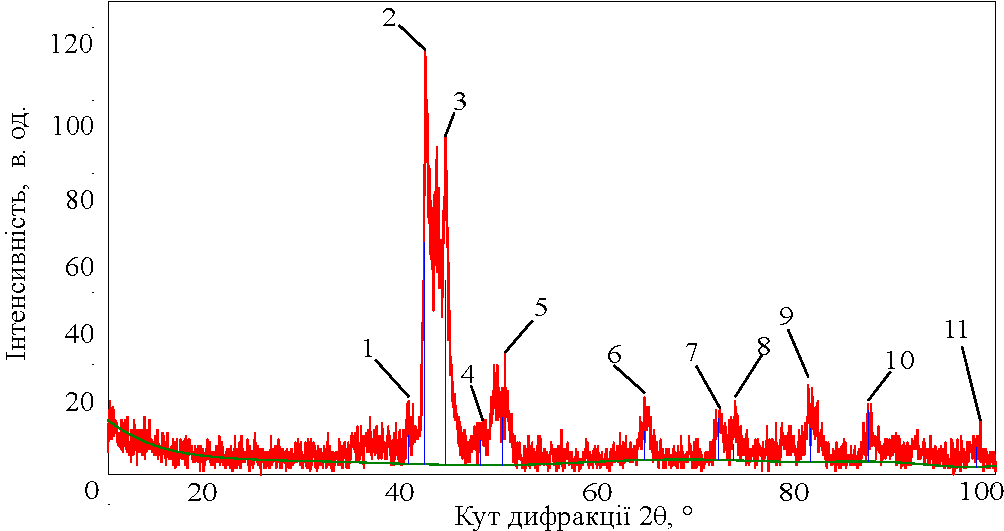
\includegraphics[width=\textwidth]{rigaku_peaks_W-C-Cr.ps}
\caption{Дифрактограма покриття W-C-Cr після ЕІЛ сталі~45}
\label{fig:peaks_W-C-Cr}
\end{figure}

Аналіз піків на дифрактограмі показав, що в зразку присутні такі фази як: Cr, WC, W\textsubscript{2}C, CrC~(табл.~\ref{tab:peaks_W-C-Cr}).

\begin{table}[H]
\centering
\caption{Фазовий склад покриття W-C-Cr після ЕІЛ сталі~45}
\label{tab:peaks_W-C-Cr}
\begin{tabular}{|l|c|c|l|c|}
  \hline
  \multicolumn{1}{|c|}{№} & \multicolumn{1}{c|}{Кут дифракції 2$\theta$, \degree} & \multicolumn{1}{c|}{Міжплощинна відстань d, \AA} &  \multicolumn{1}{c|}{Фаза} & \multicolumn{1}{c|}{HKL} \\ \hline
  1 & 40 & 2,2286 & W\textsubscript{2}C & 121 \\ \hline
  2 & 42 & 2,1442 & Cr & 111 \\ \hline
  3 & 44 & 2,0483 & CrC & 200 \\ \hline
  4 & 48 & 1,9017 & WC & 101 \\ \hline
  5 & 50 & 1,8246 & Cr & 200 \\ \hline
  6 & 64 & 1,4444 & CrC & 220 \\ \hline
  7 & 72 & 1,3115 & W\textsubscript{2}C & 302 \\ \hline
  8 & 73 & 1,2890 & WC & 111 \\ \hline
  9 & 81 & 1,1835 & Cr & 211 \\ \hline
  10 & 87 & 1,1176 & WC & 201 \\ \hline
  11 & 98 & 1,0197 & CrC & 400 \\ \hline
  \end{tabular}
\end{table}

За даними рентгеноструктурного аналізу розраховані періоди кристалічних ґраток виявлених фаз, їх параметри субструктури. Розраховані дані наведені в табл.~\ref{tab:structure_W-C-Cr}.

\begin{table}[H]
\centering
\caption{Параметри структури покриття W-C-Cr}
\label{tab:structure_W-C-Cr}
\begin{tabular}{|l|r|r|r|c|r|}
\hline
\multicolumn{1}{|c|}{\multirow{2}{*}{Фаза}} & \multicolumn{3}{c|}{Періоди ґратки, \AA} & \multicolumn{1}{c|}{\multirow{2}{*}{Розміри ОКР, \AA}} & \multicolumn{1}{c|}{\multirow{2}{*}{Мікронапруження  $\frac{\Delta d}{d}$, \%}} \\ \cline{2-4}
\multicolumn{1}{|c|}{} & \multicolumn{1}{c|}{a} & \multicolumn{1}{c|}{b} & \multicolumn{1}{c|}{c} & \multicolumn{1}{c|}{} & \multicolumn{1}{c|}{} \\ \hline

Cr & 3,7272 & -- & -- & 242,8 & 1,582 \\ \hline
W\textsubscript{2}C & 4,83 & 6,23 & 4,54 & 21,685 & 0,53 \\ \hline
WC & 2,845 & -- & 2,916 & 28,451 & 1,3212 \\ \hline
CrC & 4,076 & -- & 4,076 & 21,626 & 0,25 \\ \hline

\end{tabular}
\end{table}

Мікродюрометричним аналізом (рис.~\ref{fig:plt_hard_W-C-Cr}) виявлено, що при легуванні у послідовності W-C-Cr на повітрі найбільше значення мікротвердості становить 18,9~ГПа, що приблизно у 8~разів більше за мікротвердість cталі~45.

Було проведено  випробування на зносостійкість в умовах сухого тертя за схемою ``площина по площині'' протягом 2~годин. За отриманими даними гравіметричним методом побудована залежність інтенсивності зношування від часу випробування для зразку W-C-Cr~(рис.~\ref{fig:plt_wear_W-C-Cr}).

\begin{figure}[H]
\centering  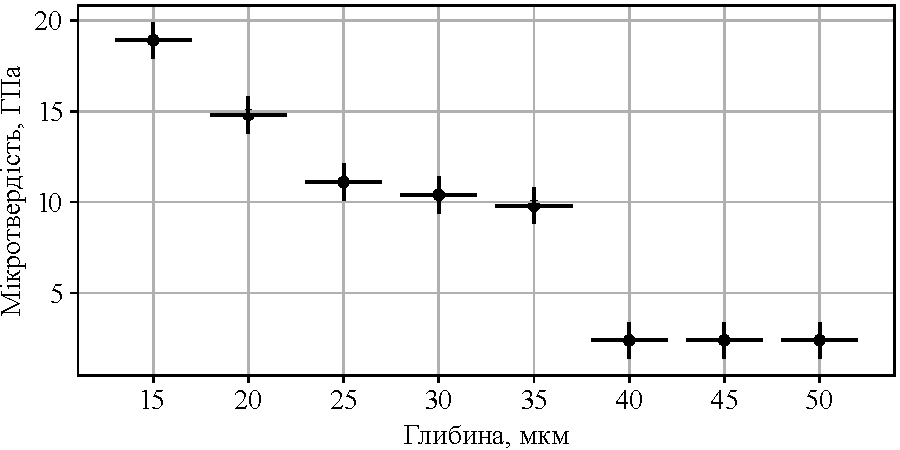
\includegraphics[]{plt_hard_W-C-Cr.pdf}
\caption{Мікротвердість повехневої зони сталі~45 після ЕІЛ за схемою W-C-Cr}
\label{fig:plt_hard_W-C-Cr}
\end{figure}

\begin{figure}[H]
\centering
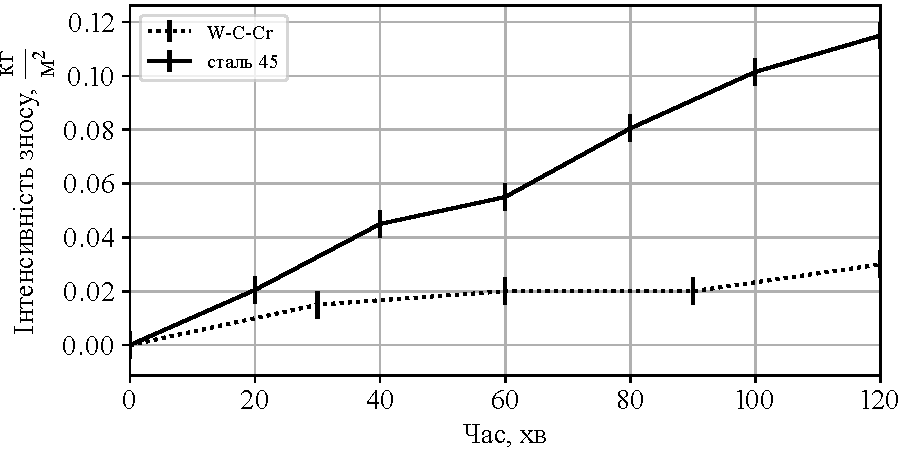
\includegraphics[]{plt_wear_W-C-Cr.pdf}
\caption{Залежність інтенсивності зносу від часу для зразку W-C-Cr}
\label{fig:plt_wear_W-C-Cr}
\end{figure}

Розраховане відношення інтенсивностей зношування сталі~45 без обробки та сформованої поверхні становить 3,8. Інтенсивність зношування починає вирівнюватися приблизно з 60-ої хвилини випробування.

\section{Формування покриття на сталі~45 під час ЕІЛ за схемою C-Cr-W}

Після ЕІЛ сталі~45 у послідовності C-Cr-W мікродюрометричним аналізом виявлено, що товщина легованого шару становить від 20~мкм до 30~мкм. Легований шар є несуцільним, на деяких ділянкам містить тріщини~(рис.~\ref{fig:adapt_microstr_C-Cr-W}).

\begin{figure}[H]
\centering
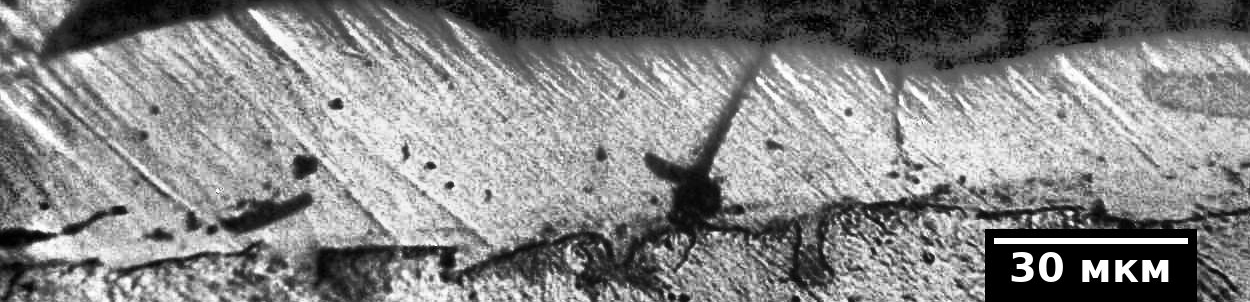
\includegraphics[width=\textwidth]{adapt_gray_microstr_C-Cr-W.jpg}
\caption{Мікроструктура поверхні сталь~45 після ЕІЛ за схемою C-Cr-W}
\label{fig:adapt_microstr_C-Cr-W}
\end{figure}

Графік кінетики масоперенесення наведений на рис.~\ref{fig:plt_gravi_C-Cr-W}.

\begin{figure}[H]
\centering 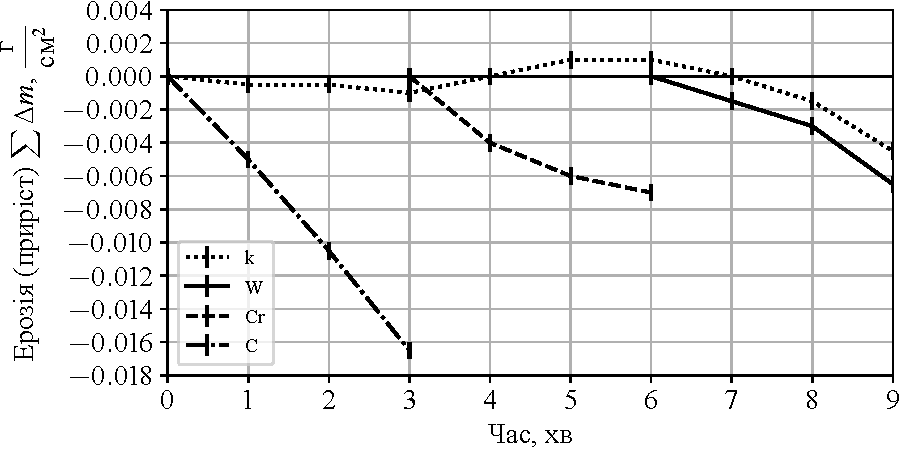
\includegraphics[]{plt_gravi_C-Cr-W.pdf}
\caption{Кінетика масоперенесення під час ЕІЛ за схемою C-Cr-W}
\label{fig:plt_gravi_C-Cr-W}
\end{figure}

В процесі легування крива приросту маси катоду зростає лише на 4-й хвилині обробки, під завершення другої стадії обробки після зміни матеріалу аноду на хром. На стадії легування вольфрамом приріст маси катоду від'ємний. Це свідчить про те, що процес легування за обраної схеми у повітряному середовищі має незначну ефективність формування покриття.

Результатом рентгенофазового аналізу є дифрактограма~(рис.~\ref{fig:peaks_C-Cr-W}), розшифровка якої наведена в таблиці~\ref{tab:peaks_C-Cr-W}.

\begin{figure}[H]
\centering
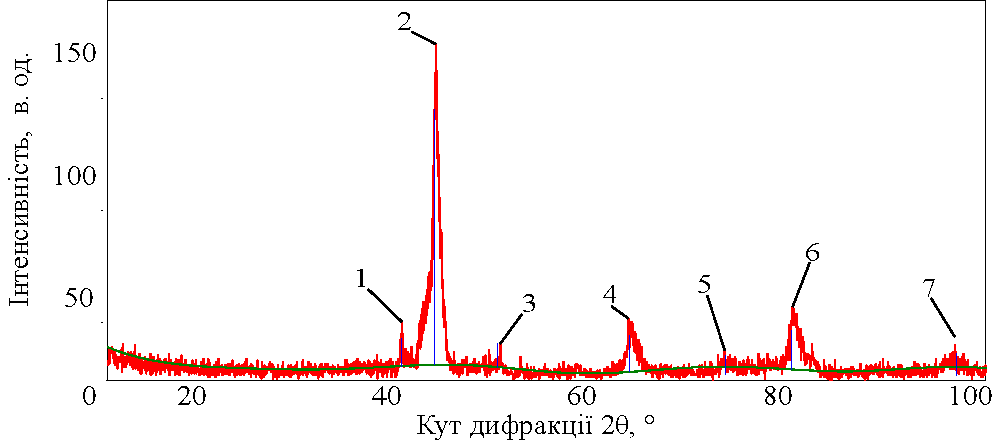
\includegraphics[width=\textwidth]{rigaku_peaks_C-Cr-W.ps}
\caption{Дифрактограма покриття C-Cr-W після ЕІЛ сталі~45}
\label{fig:peaks_C-Cr-W}
\end{figure}

\begin{table}[H]
\centering
\caption{Фазовий склад покриття C-Cr-W після ЕІЛ сталі~45}
\label{tab:peaks_C-Cr-W}
\begin{tabular}{|l|p{2cm}|c|l|c|}

  \hline
  \multicolumn{1}{|c|}{№} &
  \multicolumn{1}{c|}{Кут дифракції 2$\theta$, \degree} &
  \multicolumn{1}{c|}{Міжплощинна відстань d, \AA} &
  \multicolumn{1}{c|}{Фаза} &
  \multicolumn{1}{c|}{HKL} \\ \hline

  1 & 40 & 2,2456 & W\textsubscript{2}C & $11\bar{1}$ \\ \hline
  2 & 44 & 2,0768 & CrC & 200 \\ \hline
  3 & 50 & 1,8232 & Fe\textsubscript{3}C & 201 \\ \hline
  4 & 64 & 1,4638 & CrC & 220 \\ \hline
  5 & 73 & 1,2897 & W\textsubscript{2}C & 220 \\ \hline
  6 & 80 & 1,1977 & CrC & 220 \\ \hline
  7 & 97 & 1,0283 & Fe\textsubscript{3}C & 260 \\ \hline

  \end{tabular}
\end{table}

Фазовий аналіз показав, що в зразку присутні такі фази як: Cr, WC, W\textsubscript{2}C, CrC~(рис.~\ref{fig:peaks_C-Cr-W}, табл.~\ref{tab:peaks_C-Cr-W}).
Розраховані періоди кристалічних ґраток кожної фази, параметри субструктури (області когерентного розсіювання та мікровикривлення ґратки) наведені в табл.~\ref{tab:structure_C-Cr-W}.

\begin{table}[H]
\centering
\caption{Параметри структури покриття C-Cr-W}
\label{tab:structure_C-Cr-W}
\begin{tabular}{|l|r|r|r|c|r|}
\hline

  \multicolumn{1}{|c|}{%
    \multirow{2}{*}{Фаза}
    } &
  \multicolumn{3}{c|}{Періоди ґратки, \AA} &
  \multicolumn{1}{c|}{%
    \multirow{2}{*}{Розміри ОКР, \AA}
    } &
  \multicolumn{1}{c|}
    } \\

  \cline{2-4}

  &
  \multicolumn{1}{c|}{a} &
  \multicolumn{1}{c|}{b} &
  \multicolumn{1}{c|}{c} &
  & \\ \hline

Fe\textsubscript{3}C & 5,0442 & 6,8375 & 4,4846 & 67,13 & 0,0 \\ \hline
CrC & 4,1364 & 4,1364 & 4,1364 & 77,113 & 0,3256 \\ \hline
W\textsubscript{2}C & 5,0936 & 5,0936 & 4,7618 & 52,72 & 0,747 \\ \hline

\end{tabular}
\end{table}

За даними мікродюрометричного аналізу (рис.~\ref{fig:plt_hard_C-Cr-W}) виявлено, що при легуванні з використанням схеми C-Cr-W на повітрі найбільше значення мікротвердості становить 14,8~ГПа, що приблизно у 6~разів більше за мікротвердість cталі~45.

\begin{figure}[H]
\centering 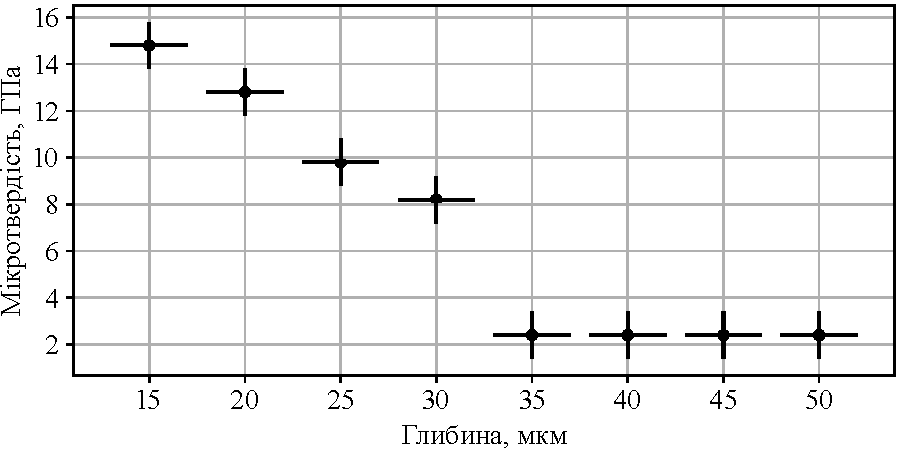
\includegraphics[]{plt_hard_C-Cr-W.pdf}
\caption{Мікротвердість повехневої зони сталі~45 після ЕІЛ за схемою C-Cr-W}
\label{fig:plt_hard_C-Cr-W}
\end{figure}

За результатами випробування на зносостійкість в умовах сухого тертя за схемою ``площина по площині'' протягом 2~годин побудована часова залежність інтенсивності зношування для зразку C-Cr-W~(рис.~\ref{fig:plt_wear_C-Cr-W}).

\begin{figure}[H]
\centering
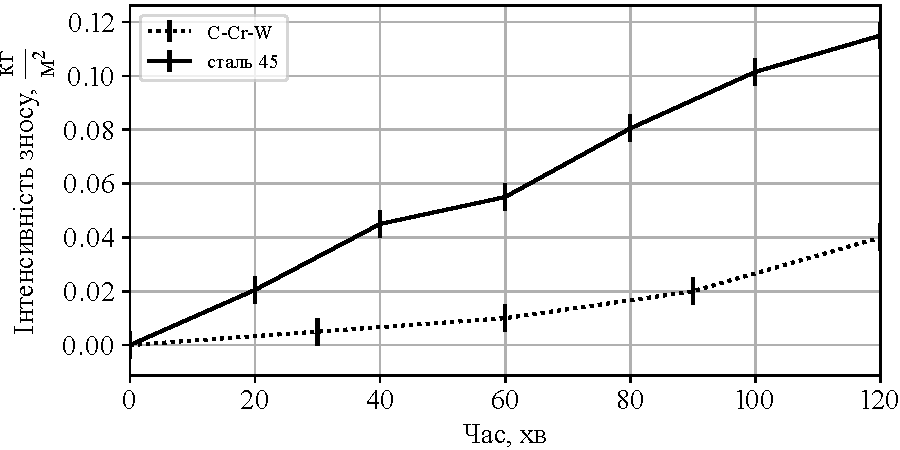
\includegraphics[]{plt_wear_C-Cr-W.pdf}
\caption{Залежність інтенсивності зносу від часу для зразку C-Cr-W}
\label{fig:plt_wear_C-Cr-W}
\end{figure}

Розраховане відношення інтенсивностей зношування даного зразка та сталі~45 становить 2,9. ``Поличка зносостійкості'' не спостерігається, інтенсивність для легованого зразку зростає на всьому проміжку часу як і крива інтенсивності зношування для сталі~45.

\section{Порівняльна характеристика}

В результаті гравіметричного аналізу в процесі легування для кожного зразка були обраховані дві константи за формулами~\eqref{eq:effectiveness_coef_x} та~\eqref{eq:effectiveness_coef_cr}, за допомогою яких можна оцінити ефективність утворення легованого шару за процесу ЕІЛ~(рис.~\ref{fig:comp_grav}).

\begin{figure}[H]
\centering
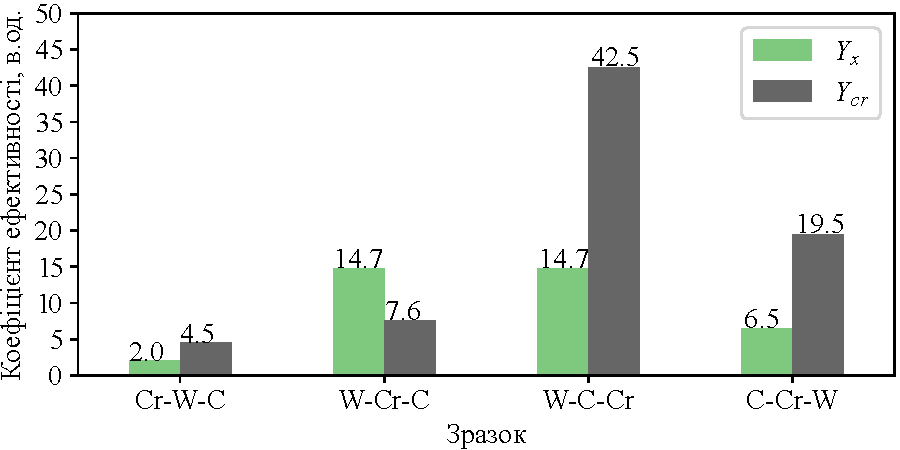
\includegraphics[]{comp_grav.pdf}
\caption{Коефіцієнти ефективності утворення легованого шару}
\label{fig:comp_grav}
\end{figure}

За результатами отриманих даних по зразкам Cr-W-C, W-Cr-C, W-C-Cr, C-Cr-W було проведено порівняння властивостей мікротвердості, зносостійкості з відповідними властивостями сталі~45 без обробки ЕІЛ~(рис.~\ref{fig:comp_wh}).

З оброблених схем легування максимальну зносостійкість у порівнянні з необробленим зразком сталі~45 була отримана за схемою Cr-W-C, яка має найменше збільшення за мікротвердістю. При цьому найбільше відношення мікротвердості відповідає зразку W-C-Cr.


\begin{figure}[H]
\centering
\vspace{-0.5cm}
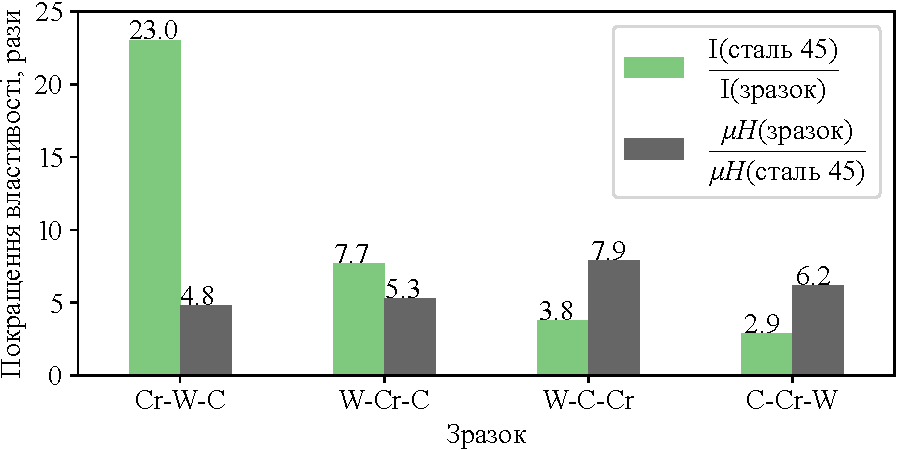
\includegraphics[]{comp_wh.pdf}
\caption{Порівняння максимальної мікротвердості та інтенсивності зносостійкості з відповідними значеннями для сталі~45 без обробки}
\label{fig:comp_wh}
\end{figure}



\section{Висновки до розділу~\thechapter}

Встановлено вплив послідовності стадій електроіскрового легування з використанням вольфрамового, графітового та хромового анодів на структуру, мікротвердість та зносостійкість покриттів на сталі~45.

Проведені експериментальні дослідження, які показують, що для ЕІЛ на сталі~45 за схемами W-C-Cr, C-Cr-W, W-Cr-C, Cr-W-C можливе утворення легованого шару товщиною від 15~мкм до 30~мкм.

Встановлено підвищення поверхневої мікротвердості сталі~45 у діапазоні від \SIrange{11.5}{18.9}{\gpa} після нанесення електроіскрових покриттів за всіма запропонованими схемами за рахунок наявності твердих розчинів матеріалів електродів та  карбідів WC, W\textsubscript{2}C, Fe\textsubscript{3}C, CrC, Cr\textsubscript{3}C\textsubscript{2}.

Виявлено, що зносостійкість покриттів зростає в ряду C-Cr-W $\rightarrow$ W-C-Cr $\rightarrow$ W-Cr-C $\rightarrow$ Cr-W-C від 3~разів до 23~разів у порівнянні з необробленою поверхнею сталі~45.

Розрахована ефективність формування шарів за результатами гравіметричного аналізу: для схеми нанесення W-C-Cr вона складає~--- 42,5; для C-Cr-W~--- 19,5; для W-Cr-C~--- 14,7; для Cr-W-C~--- 4,5.


\chapter{ОРГАНІЗАЦІЙНO-ЕКОНОМІЧНА ЧАСТИНА}
\label{chap:economics}

\section{Науково-технічна актуальність НДР}

В галузі машинобудування та металообробки важливим питанням є доцільність того чи іншого технологічного процесу. Наприклад для дорогих та дефіцитних марок сталей, що застосовуються при виготовленні інструменту і деталей машин, використовують різні функціональні покриття, що можуть забезпечити довговічність та надійність деталей машин або інструменту. Властивості покриттів можна варіювати за допомогою підбору методу нанесення, режиму та легуючих елементів.

Розглянутий в роботі метод електроіскрового легування дозволяє виконувати такі операції створення покриття без особливої складності технології проведення~\cite{hitlevich1985}. Звісно процес має опцію ускладнення --- проведення ЕІЛ в насичуючих середовищах. Але в роботі не розглядається дана можливість, так як метою є дослідження отриманої поверхні з варіюванням послідовності анодних матеріалів в стадіях легування.

З економічної точки зору перевагами ЕІЛ є те, що дана обробка є простою за виконанням та енергетично вигідна~\cite{liu2007}. Важливою умовою лише є наявність однофазного струму.

\section{Мета і завдання НДР}

Метою даної роботи було формування функціональних покриттів на сталі~45 багатостадійним електроіскровим легуванням хромом, вольфрамом та графітом. Завданнями даної роботи були:
\begin{itemize}
\item опрацювання фахових публікацій з даного напряму;
\item розробка методики дослідження;
\item виготовлення і обробка зразків;
\item проведення ЕІЛ;
\item виготовлення мікрошліфів;
\item дослідження властивостей (мікротвердість, мікроструктура і фазовий склад) отриманого поверхневого шару;
\item аналіз залежності властивостей поверхневого шару від кількості стадій обробки;
\item формулювання висновків по роботі та надання відповідних рекомендацій.
\end{itemize}

\section{Розрахунок планових витрат на проведення НДР}

Робота виконувалася на кафедрі Фізики металів у КПІ імені Ігоря Сікорського. Планова кошторисна вартість (собівартість) НДР розраховувалась у відповідності до таких калькуляційних статтей витрат:
\begin{itemize}
\item заробітна плата науково-виробничого персоналу;
\item єдиний соціальний внесок;
\item вартість матеріалів, необхідних для виконання НДР;
\item вартість спеціального обладнання для проведення експерименту;
\item службові відрядження;
\item інші прямі невраховані витрати;
\item накладні витрати.
\end{itemize}

\subsection{Витрати на оплату праці}
\label{subsec:salary}

У виконанні НДР брали участь чотири виконавці: провідний науковий співробітник, старший науковий співробітник та інженер дослідник. Для КПІ ім.~Ігоря~Сікорського тарифні ставки сумарної місячної заробітної плати складають:
\begin{itemize}
\item провідного наукового співробітника --- \SI{10944}{\grn};
\item старшого наукового співробітника --- \SI{9600}{\grn};
\item інженера-дослідника --- \SI{5824}{\grn}.
\end{itemize}

Денна заробітна плата кожного з виконавців визначається як місячна заробітна плата, поділена на середню кількість днів у місяці, що при п'ятиденному робочому тижні становить~21,2. Таким чином, величина денної заробітної плати виконавців складає:
\begin{itemize}
\item для провідного наукового співробітника --- \SI{516.23}{\grn};
\item старшого наукового співробітника --- \SI{452.82}{\grn};
\item інженера-дослідника --- \SI{274.72}{\grn}.
\end{itemize}

У випадку відсутності відповідних розрахункових методик трудомісткість різних етапів виконання НДР встановлюється на базі експертних оцінок, які дають провідні фахівці. При цьому НДР розглядається як сукупність макроетапів, аналіз кожної окремої операції не проводиться. Результати експертної оцінки трудомісткості етапів НДР наведені в табл.~\ref{tab:labor_hours}.

% Please add the following required packages to your document preamble:
% \usepackage{multirow}
\begin{table}[H]
\centering
\caption{Трудомісткість макроетапів виконання НДР}
\label{tab:labor_hours}
\begin{tabular}{|l|c|c|c|}
\hline
\multicolumn{1}{|c|}{\multirow{2}{*}{\begin{tabular}[c]{@{}c@{}}Макроетапи\\ 				НДР\end{tabular}}} & \multicolumn{3}{c|}{\begin{tabular}[c]{@{}c@{}}Трудомісткість\\ 				за виконавцями, люд.-дні\end{tabular}} \\ \cline{2-4}
\multicolumn{1}{|c|}{} & \begin{tabular}[c]{@{}c@{}}Провідний\\ науковий\\ співробітник\end{tabular} & \begin{tabular}[c]{@{}c@{}}Старший\\ науковий\\ співробітник\end{tabular} & \begin{tabular}[c]{@{}c@{}}Інженер-\\ дослідник\end{tabular} \\ \hline
\begin{tabular}[c]{@{}l@{}}1. Аналіз фахових публікацій\\ за темою та обгрунтування\\ мети та напрямів, дослідження\end{tabular} & 14 & 12 & 0 \\ \hline
\begin{tabular}[c]{@{}l@{}}2. Розробка методики\\ проведення досліджень\\ за темою\end{tabular} & 3 & 2 & 1 \\ \hline
\begin{tabular}[c]{@{}l@{}}3. Проведення експерименту\\ 				3.1. Виготовлення зразків\\ 				3.2. Проведення ЕІЛ\\ 				3.3. Дослідження властивостей\end{tabular} & 2 & 2 & 2 \\ \hline
5. Обговорення результатів НДР & 14 & 12 & 0 \\ \hline
Всього & 33 & 28 & 3 \\ \hline
\end{tabular}
\end{table}


Величина фонду заробітної плати виконавців (ФЗП) обчислюється як сума добутків трудомісткості і денної заробітної плати кожного з них:
\begin{equation*}
  \text{ФЗП} = \SI{30538.87}{\grn}.
\end{equation*}

\subsection{Визначення розміру єдиного соціального внеску}
%\label{subsec:label}

Згідно з діючим законодавством єдиний соціальний внесок становить \SI{22}{\%} від фонду заробітної платні:
\begin{equation*}
\text{В}_{\text{C}} = 0,22 \cdot \text{ФЗП} = 6~718,55 \text{ грн}.
\label{eq:social}
\end{equation*}

\subsection{Визначення вартості матеріалів для виконання НДР}

Для проведення досліджень використовувались наступні матеріали: зразки із сталі~45 та відповідні електроди. Дані про вартість перелічених матеріалів наведені в таблиці~\ref{tab:material_costs}.

\begin{table}[H]
\centering
\caption{Вартість основних матеріалів}
\label{tab:material_costs}
\begin{tabular}{|l|c|c|c|c|}
\hline
\multicolumn{1}{|c|}{Найменування} & \begin{tabular}[c]{@{}c@{}}Одиниця\\ вимірювання\end{tabular} & Кількість & \begin{tabular}[c]{@{}c@{}}Ціна,\\ грн.\end{tabular} & \begin{tabular}[c]{@{}c@{}}Сума, \\ грн.\end{tabular} \\ \hline
  Зразок сталь~45&шт.&4&6&24\\\hline
  Електрод W&шт.&1&12&12\\\hline
  Електрод C&шт.&1&2&2\\\hline
  Електрод Cr&шт.&1&8&8\\\hline
  \multicolumn{4}{|l|}{Всього} &46\\ \hline
\end{tabular}
\end{table}

Транспортно-заготівельні витрати приймаємо у розмірі 10\% від вартості матеріалів, тоді загальні витрати по цій статті складуть:
\begin{equation*}
\text{См}= 46 \cdot 1,1 = 50,60~\text{грн}.
\end{equation*}

\subsection{Визначення вартості спеціального обладнання і приладів}
%\label{subsec:label}

При виконанні НДР усі роботи проводилися з використанням лише наявного обладнання в лабораторіях КПІ ім.~Ігоря~Сікорського.

\subsection{Визначення вартості робіт і послуг сторонніх організацій}
%\label{subsec:label}

У виконанні даної НДР сторонні організації не брали участі.

\subsection{Визначення витрат на службові відрядження}

Усі роботи, пов’язані з виконанням НДР за даною темою, проведені в лабораторіях КПІ ім.~Ігоря~Сікорського. Окремі службові відрядження не планувались.

\subsection{Визначення інших прямих неврахованих витрат по темі}

Інші прямі невраховані витрати ($\text{С}_{\text{інш}}$) плануються у розмірі 10\% від врахованих:
\begin{equation*}
\text{С}_{\text{інш}}=(30~538,87+6~718,55+50,60)\cdot 0,1 = 3~730,80~\text{грн}.
\end{equation*}

\subsection{Визначення накладних витрат}

До накладних витрат відносяться витрати на заробітну плату адміністра-тивно-управлінського, господарчого та допоміжного персоналу (разом з єдиним соціальним внеском), витрати на допоміжні виробництва, витрати на утримання та експлуатацію виробничих площ, наукових приладів та установок, витрати на охорону праці, техніку безпеки та екологію, фінансування підготовки кадрів, воєнізованої охорони і деякі інші.

Норматив відрахувань на накладні витрати для КПІ ім.~Ігоря~Cікорського встановлений в розмірі 20\% планової суми всіх прямих витрат на виконання НДР. Розраховуємо величину накладних витрат таким чином:
\begin{equation*}
\text{Н}_{\text{В}} = 0,2 \cdot (30~538,87+6~718,55+50,60+3~730,80)= 8~207,76~\text{грн}.
\end{equation*}

\subsection{Визначення планової кошторисної вартості НДР}

\enlargethispage{1\baselineskip}
Планова кошторисна вартість НДР визначається як сума витрат за окремими статтями калькуляції. Результати визначення вартості наведені у таблиці~\ref{tab:plan_calculation}.

% Please add the following required packages to your document preamble:
% \usepackage{multirow}
\begin{table}[H]
\centering
\caption{Калькуляція планової кошторисної вартості НДР за темою}
\label{tab:plan_calculation}
\begin{tabular}{|l|l|c|c|}
\hline
\multicolumn{1}{|c|}{\multirow{2}{*}{Найменування калькуляційних статей}} & \multicolumn{1}{c|}{\multirow{2}{*}{Позначення}} & \multicolumn{2}{c|}{Сума} \\ \cline{3-4}
\multicolumn{1}{|c|}{} & \multicolumn{1}{c|}{} & грн. & \% \\ \hline
  1. Фонд заробітної плати & ФЗП & 30~538,87 & 62,01 \\ \hline
  2. Єдиний соціальний внесок & ВС & 6~718,55 & 13,64 \\ \hline
  3. Матеріали, необхідні для виконання теми & $\text{С}_{\text{М}}$ & 50,60 & 0,10 \\ \hline
  4. Спеціальне обладнання для наукових робіт & $\text{С}_{\text{об}}$ & ─ & ─ \\ \hline
  5. Робота і послуги сторонніх організацій & $\text{С}_{\text{стор}}$ & ─ & ─ \\ \hline
  6. Витрати на службові відрядження & $\text{С}_{\text{від}}$ & ─ & ─ \\ \hline
  7. Інші прямі невраховані витрати & $\text{С}_{\text{інш}}$ & 3~730,80 & 7,58 \\ \hline
  8. Накладні витрати & $\text{Н}_{\text{В}}$ & 8~207,76 & 16,67 \\ \hline
\multicolumn{2}{|l|}{Всього} & 49~246,59 & 100,00 \\
\hline
\end{tabular}
\end{table}


Відповідно до табл.~\ref{tab:plan_calculation} загальна планова кошторисна вартість НДР складає $\text{В}_{\text{НДР}}=49~246,59~\text{грн}$.

\section{Науково-технічна ефективність НДР}

Дана робота має пошуковий та теоретичний характер. Відповідно до цього прямий розрахунок очікуваного річного економічного ефекту складний, оскільки відсутні повні дані відносно сфери використання результатів роботи, а також вихідні дані для розрахунку єдиночасних та поточних витрат. У такому випадку слід використовувати бальну систему оцінки економічної ефективності за наступними показниками:
\begin{itemize}
\item важливість розробки ($K_1$);
\item можливість використання результатів ($K_2$);
\item теоретичне значення та рівень новизни дослідження ($K_3$);
\item складність розробки ($K_4$).
\end{itemize}

Коефіцієнт $K_1$ може приймати наступні значення:
\begin{itemize}
\item ініціативна робота, яка не входить до складу комплексної програми та не є завданням директивних органів~--- 1 бал;
\item робота виконується за угодою про науково-технічне співробітництво~--- 3 бали;
\item робота являє собою частину відомчої програми~--- 5 балів;
\item робота являє собою частину комплексної міжвідомчої програми з елементами впровадження результатів~--- 7 балів;
\item робота є частиною міжнародної комплексної програми~--- 8 балів.
\end{itemize}

Коефіцієнт $K_2$ може приймати такі значення:
\begin{itemize}
\item результати розробки можна використати тільки в даному підрозділі~--- 1 бал;
\item результати розробки можуть бути використані тільки однією організацією~--- 3 бали;
\item результати розробки можуть бути використані багатьма організаціями~--- 5 балів.
\item результатами розробки можуть користуватися споживачі в межах однієї галузі~--- 8 балів;
\item результатами розробки можуть користуватися споживачі в різних галузях~--- 10 балів.
\end{itemize}

Коефіцієнт $K_3$ може приймати такі значення:
\begin{itemize}
\item робота являє собою аналіз, узагальнення або класифікацію відомої інформації, подібні результати раніше були відомі в досліджуваній галузі~--- 2 бали;
\item під час виконання роботи отримана нова інформація, яка доповнює уявлення про сутність досліджуваних процесів~--- 3 бали;
\item внаслідок виконання роботи отримана нова інформація, яка частково змінює уявлення про природу досліджуваних процесів~--- 5 балів;
\item внаслідок виконання НДР створені нові теорії, методики або що-небудь подібне~--- 6 балів;
\item отримана інформація формує принципово нові уявлення, які не були відомі раніше~--- 8 балів.
\end{itemize}

Коефіцієнт $K_4$ може приймати такі значення:
\begin{itemize}
\item роботу виконує один підрозділ, витрати до 10~000~грн --- 1 бал;
\item роботу виконує один підрозділ, витрати від 10~000~грн до 50~000~грн --- 3 бали;
\item роботу виконує один підрозділ, витрати від 50~000~грн до 100~000~грн --- 5 балів;
\item робота виконується багатьма підрозділами, витрати від 100~000~грн до 200~000~грн --- 7 балів;
\item робота виконується багатьма організаціями, витрати більше 200~000~грн --- 9 балів.
\end{itemize}

Бальна оцінка економічної ефективності даної науково-дослідної роботи наведена у табл.~\ref{tab:econom_efficiency_coef}.

\begin{table}[H]
\centering
\caption{Бальна оцінка ефективності НДР}
\label{tab:econom_efficiency_coef}
\begin{tabular}{|l|l|l|l|}
\hline
\multicolumn{1}{|c|}{\begin{tabular}[c]{@{}c@{}}Показники оцінки\\ ефективності НДР\end{tabular}} & \multicolumn{1}{c|}{\begin{tabular}[c]{@{}c@{}}Умовне\\ позначення\\ показника\end{tabular}} & \multicolumn{1}{c|}{\begin{tabular}[c]{@{}c@{}}Характеристика\\ даної розробки\end{tabular}} & \multicolumn{1}{c|}{\begin{tabular}[c]{@{}c@{}}Кількість\\ балів\end{tabular}} \\ \hline
\begin{tabular}[c]{@{}l@{}}1. Важливість\\ розробки\end{tabular} & К1 & \begin{tabular}[c]{@{}l@{}}Робота ініціативна,\\ не є завданням\\ будь-яких директивних\\ органів або частиною\\ комплексної програми\end{tabular} & 1 \\ \hline
\begin{tabular}[c]{@{}l@{}}2. Можливість\\ використання\\ результатів\\ розробки\end{tabular} & К2 & \begin{tabular}[c]{@{}l@{}}Результати розробки\\ можуть бути\\ використані багатьма\\ організаціями\end{tabular} & 8 \\ \hline
\begin{tabular}[c]{@{}l@{}}3. Теоретична\\ значимість\\ та рівень новизни \\ розробки\end{tabular} & К3 & \begin{tabular}[c]{@{}l@{}}Отримання нової інформації,\\ яка доповнює уявлення про\\ сутність досліджуваних\\ процесів та була невідома\\ раніше\end{tabular} & 5 \\ \hline
\begin{tabular}[c]{@{}l@{}}4.Складність\\ проведення\\ дослідження\end{tabular} & К4 & \begin{tabular}[c]{@{}l@{}}Робота виконується одним\\ підрозділом, витрати\\ від 10~000~грн до 50~000 грн\end{tabular} & 3 \\ \hline
\end{tabular}
\end{table}

\enlargethispage{1\baselineskip}
Загальна бальна оцінка ефективності згідно з табл.~\ref{tab:econom_efficiency_coef} становить:
\begin{equation*}
\text{Б} = K_1 \cdot K_2 \cdot K_3 \cdot K_4= 1 \cdot 8 \cdot 5 \cdot 3 = 120.
\end{equation*}

Умовний річний економічний ефект ($\text{ЕНДР}$) науково-дослідницької роботи визначається:
\begin{equation}
\text{Е}_{\text{НДР}} = 500 \cdot \text{Б} - \text{Е}_{\text{н}} \cdot \text{В}_{\text{НДР}},
\label{eq:econom_eff}
\end{equation}
\begin{eqitemize}
\item[де] 500 --- умовна вартість одного балу, грн.;
\item $\text{Е}_{\text{н}}$ --- нормативний коефіцієнт економічної ефективності ($\text{Е}_{\text{н}} = 0,15 \cdot 0,5$, для нашого розрахунку обираємо $\text{Е}_{\text{н}} = 0,2$);
\item $\text{В}_{\text{НДР}}$ --- витрати на виконання НДР (планова річна кошторисна вартість виконання НДР, для нашого розрахунку $\text{В}_{\text{НДР}}= 49~246,59~\text{грн}.$).
\end{eqitemize}

Таким чином, умовний економічний ефект відповідно (\ref{eq:econom_eff}) становить:
\begin{equation*}
\text{Е}_{\text{НДР}}=500 \cdot 120 - 0,2 \cdot 49~246,59 = 50~150,68~\text{грн}.
\end{equation*}

Коефіцієнт економічної ефективності:
\begin{equation*}
\text{К}_{\text{НДР}}= \frac{\text{Е}_{\text{НДР}}}{\text{В}_{\text{НДР}}}= 1,02
\end{equation*}

Отримана розрахункова величина коефіцієнта економічної ефективності НДР більше одиниці, що свідчить про доцільність виконання даної роботи.

\section{Висновки до розділу~\thechapter}

Отже була обґрунтована науково-технічна актуальність виконання досліджень по даній темі. Розрахована планова річна собівартість проведення науково-дослідної роботи, яка становить 49~246,59~грн. При цьому коефіцієнт умовної економічної ефективності проведення роботи становить~1,02. З цього слідує, що проведення НДР є економічно доцільним.

\chapter{ОХОРОНА ПРАЦІ}
\label{chap:work_safety}

\section{Вступ}

Охорона праці --- це система правових, соціально-економічних, організа-ційно-технічних, санітарно-гігієнічних і лікувально-профілактичних заходів та засобів, спрямованих на збереження життя, здоров'я і працездатності людини під час її трудової діяльності~\cite{tkachuk2006}.

Законодавство в сфері працевлаштування регулює трудові відносини працівників усіх підприємств, установ, організацій незалежно від форм власності, виду діяльності та галузі роботи, а також осіб, які працюють згідно з трудовим договором з фізичною особою. Нагляд за дотриманням норм охорони праці є одним із обов'язків прокуратури~(загальний нагляд) та професійних спілок~(спеціальний нагляд). Також даний контроль можуть здійснювати державні та відомчі спеціалізовані інспекції.~\cite{tkachuk2006}

Метою розділу є  аналіз шкідливих та небезпечних факторів та умов, за яких можливе ураження або травмування організму в процесі дослідження функціональних покриттів на поверхні сталі~45, які були нанесені багатостадійним електроіскровим легуванням, а також розробка заходів спрямованих на усунення цих факторів та вивчення безпеки у надзвичайних ситуаціях.

\section{Правові та організаційні основи охорони праці на підприємстві}

Законодавство України про охорону праці --- це система взаємозв’язаних законів та інших нормативно-правових актів, що регулюють відносини у сфері реалізації державної політики щодо соціального захисту її громадян в процесі трудової діяльності. Воно складається з Закону України <<Про охорону праці>>, Кодексу законів про працю України, Закону України <<Про загальнообов’язкове державне соціальне страхування від нещасного випадку на виробництві та професійного захворювання, які спричинили втрату працездатності>> та прийнятих відповідно до них нормативно-правових актів.~\cite{tkachuk2006}

%Базується законодавство України про охорону праці на конституційному праві всіх громадян України на належні, безпечні і здорові умови праці, гарантовані статтею~43 Конституції України. Стаття~45 Конституції гарантує право всіх працюючих на щотижневий відпочинок та щорічну оплачувану відпустку, а також встановлення скороченого робочого дня щодо окремих професій і виробництв, скороченої тривалості роботи у нічний час.

%Основоположним документом в галузі охорони праці є Закон України <<Про охорону праці>>, який визначає основні положення щодо реалізації конституційного права працівників на охорону їх життя і здоров’я у процесі трудової діяльності, на належні, безпечні і здорові умови праці, регулює за участю відповідних державних органів відносини між роботодавцем і працівником з питань безпеки, гігієни праці та виробничого середовища і встановлює єдиний порядок організації охорони праці в Україні. Інші нормативні акти мають відповідати не тільки Конституції та іншим законам України, але, насамперед, цьому Законові.~\cite{tkachuk2006}

Відповідно до статті~13~\cite{law_aboutwork1992} Закону України <<Про охорону праці>> роботодавець зобов'язаний створити на робочому місці в кожному структурному підрозділі умови праці відповідно до нормативно-правових актів, а також забезпечити додержання вимог законодавства щодо прав працівників у галузі охорони праці~\cite{tkachuk2006}. З цією метою роботодавець забезпечує функціонування системи управління охороною праці і несе безпосередню відповідальність за порушення зазначених вимог.

Згідно зі статтею~14~\cite{law_aboutwork1992} Закону України <<Про охорону праці>> працівник зобов'язаний: дбати про особисту безпеку і здоров'я, а також про безпеку і здоров'я оточуючих людей в процесі виконання будь-яких робіт чи під час перебування на території підприємства; знати і виконувати вимоги нормативно-правових актів з охорони праці, правила поводження з  устаткуванням та засобами виробництва, користуватися засобами колективного та індивідуального захисту; проходити у встановленому законодавством порядку попередні та періодичні медичні огляди. Працівник несе безпосередню відповідальність за порушення зазначених вимог.

Відповідно до статті~15~\cite{law_aboutwork1992} Закону України <<Про охорону праці>> на підприємстві з кількістю працюючих 50 і більше осіб роботодавець створює службу охорони праці відповідно до типового положення, що затверджується центральним органом виконавчої влади з питань нагляду за охороною праці.

Припис спеціаліста з охорони праці може скасувати лише роботодавець. Ліквідація служби охорони праці допускається тільки у разі ліквідації підприємства чи припинення використання найманої праці фізичною особою~\cite{tkachuk2006}.

Служба охорони праці підпорядковується ректору КПІ ім.~Ігоря~Cікорського М.З.~Згуровському. Очільник відділу охорони праці в КПІ ім.~Ігоря~Cікорського --- Е.Г.~Луцик. Відповідальний за охорону праці в КПІ ім.~Ігоря~Cікорського --- М.М.~Полторацький, на інженерно-фізичному факультеті --- Лобода~П.І., на кафедрі фізики металів --- С.Б.~Васільєв. В лабораторії~036-09, де виконувалась робота відповідальним за охорону праці є А.І~Мазур.

\section{Аналіз параметрів приміщення}

Дослідження проводилось на кафедрі фізики металів КПІ ім.~Ігоря~Cікорського в лабораторії електроіскрового легування 036-09. Схематичне зображення лабораторії, а також розташування всіх елементів представлено на рис.~\ref{fig:schema_room}.

\begin{figure}[H]
\centering
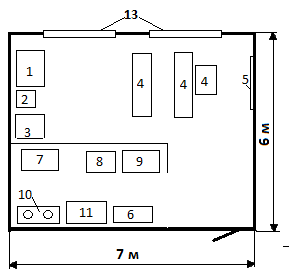
\includegraphics[width=0.4\textwidth]{schema_room.png}
\fnote{1~---~твердомір ПМТ-3; 2~---~тумба; 3~---~комп’ютер; 4~---~робочі столи; 5~---~дошка; 6~---~шафа; 7~---~стіл для шліфування; 8~---~прилад для вимірювання зносостійкості; 9~---~прилад <<Элитрон-26А>>; 10~---~полірувальні круги; 11~---~стіл}
\caption{Схематичне зображення розташування робочих елементів в лабораторії~036-09}
\label{fig:schema_room}
\end{figure}

Було проведено вимірювання параметрів приміщення лабораторії та розрахунки площі і об’єму, що припадають на одну особу. Розрахунки наведені  в табл.~\ref{tab:room}.


Згідно зі СНиП~2.09.04-87~\cite{snip} норма площі на одну особу становить 4,5~{м}${}^{2}$, а норма об'єму приміщення на одну особу~---~15~{м}${}^{3}$. Отже, з цього слідує, що лабораторія 036-09 відповідає нормам.
\begin{table}[H]
\centering
\caption{Параметри науково-дослідної лабораторії}
\label{tab:room}
\begin{tabular}{|l|r|}
\hline
\multicolumn{1}{|c|}{Характеристика} & \multicolumn{1}{c|}{Виміряні дані} \\ \hline
Довжина, м & 7 \\ \hline
Ширина, м & 6 \\ \hline
Висота, м & 3,8 \\ \hline
Площа, м$^{2}$ & 42 \\ \hline
Об’єм м$^{3}$ & 159,6 \\ \hline
Площа на одну особу, м$^{2}$ & 6 \\ \hline
Об’єм на одну особу м$^{3}$ & 42 \\ \hline
\end{tabular}
\end{table}


Для забезпечення оптимального мікроклімату <<Санітарні норми мікроклімату виробничих приміщень>> ДСН~3.3.6.042-99~\cite{dsn:microclimate} встановлюють оптимальні і допустимі значення температури, відносної вологості та швидкості руху повітря в робочій зоні в залежності від пори року та категорії важкості робіт~\cite{gelibo2001}.

Згідно з ДСН 3.3.6.042-99 категорія важкості робіт в даному дослідженні --- І~б. Відповідно до даної категорії енерговитрати оргранізму можуть бути до 150~Ккал/год.

Результати дослідження та нормовані величини параметрів мікроклімату в робочій зоні лабораторії~036-09 та їх порівняння з допустимими та оптимальними нормами наведені в табл.~\ref{tab:climate}.

\begin{table}[H]
  \centering
  \caption{Оптимальні та допустимі мікрокліматичні умови}
  \label{tab:climate}
  \begin{tabular}{|c|c|c|c|c|}
    \hline
\multicolumn{1}{|c|}{\begin{tabular}[c]{@{}c@{}}Період\\року\end{tabular}}&
\multicolumn{1}{c|}{\begin{tabular}[c]{@{}c@{}}Категорія\\робіт\end{tabular}}&
\multicolumn{1}{c|}{\begin{tabular}[c]{@{}c@{}}$t, {+}^{\circ}C$\end{tabular}}&
\multicolumn{1}{c|}{\begin{tabular}[c]{@{}c@{}}Відносна \\вологість, \%\end{tabular}}&
\multicolumn{1}{c|}{\begin{tabular}[c]{@{}c@{}}Швидкість \\руху пов., $\frac{\text{м}}{\text{с}}$\end{tabular}}\\
    \hline
    Холодний&I~б&
\multicolumn{1}{c|}{\begin{tabular}[c]{@{}c@{}}Оптимальні:\\21-23\\Допустимі:\\17-25\end{tabular}}&
\multicolumn{1}{c|}{\begin{tabular}[c]{@{}c@{}}Оптимальні:\\40-60\\Допустимі:\\до 75\end{tabular}}&
\multicolumn{1}{c|}{\begin{tabular}[c]{@{}c@{}}Оптимальні:\\0,1\\Допустимі:\\до 0,2\end{tabular}}\\
%40-60&0,1\\
    \hline
    Теплий&I~б&
\multicolumn{1}{c|}{\begin{tabular}[c]{@{}c@{}}Оптимальні: \\22-24\\Допустимі: \\19-30\end{tabular}}&
\multicolumn{1}{c|}{\begin{tabular}[c]{@{}c@{}}Оптимальні:\\40-60\\Допустимі:\\60\end{tabular}}&
\multicolumn{1}{c|}{\begin{tabular}[c]{@{}c@{}}Оптимальні:\\0,2\\Допустимі:\\0,1-0,3\end{tabular}}\\
    \hline
    Отримані дані&I~б&
\multicolumn{1}{c|}{\begin{tabular}[c]{@{}c@{}}Холодний: \\10\\Теплий: \\15\end{tabular}}&
\multicolumn{1}{c|}{\begin{tabular}[c]{@{}c@{}}Холодний:\\70\\Теплий:\\60\end{tabular}}&
\multicolumn{1}{c|}{\begin{tabular}[c]{@{}c@{}}Холодний:\\0,1\\Теплий:\\0,2\end{tabular}}\\
    \hline
  \end{tabular}
\end{table}

Оптимальним нормам в холодну пору не відповідають температурний режим та відносна вологість, в теплу пору --- лише температурний режим. Також температура в обидві пори не відповідають допустимим нормам.

Таким чином можна зробити висновок, що мікроклімат в лабораторії не повністю відповідає вимогам санітарних норм і потрібно провести заходи по поліпшенню температурного режиму. Наприклад: утеплення вікон, використання електрифікованих обігрівальних систем.




\section{Аналіз освітленості приміщення}

Розрізняють освітлення трьох видів: природнє, штучне та суміщене. Природне у свою чергу поділяється на верхнє, бічне та комбіноване. Штучне буває місцевим і загальним.~\cite{tkachuk2006}

До проблем можна віднести недостатню або надмірну освітленість та нерівномірність освітлення.  Це може призводити до зниження продуктивності праці, що зазвичай призводить до зростання потенційної небезпеки помилкових дій і нещасних випадків.

У лабораторії здійснюється природне бокове освітлення (вікна з північного боку) та штучне. Відстань від вікна до місця основної роботи складає 1~м. Для місцевого освітлення використовуються лампи розжарювання, для загального --- люмінесцентні~ЛБ-40 (24 одиниці у лабораторії)~\cite{snip}.

Для забезпечення нормованих значень освітленості в приміщенні потрібно проводити очищення скла, віконних рам і світильників не рідше двох разів у рік, а також проводити своєчасну заміну перегорілих ламп.
дмірна яскравість джерел світла може спричинити головний біль, різь в очах, розлад гостроти зору; світлові відблиски --- тимчасове засліплення. Отже освітлення, що забезпечує нормальні зорові роботи, є важливим чинником в організації і проведенні НДР.

У лабораторії здійснюється природне бокове освітлення (вікна з північного боку) та штучне. Відстань від вікна до місця основної роботи складає 1~м. Для місцевого освітлення використовуються лампи розжарювання, для загального – люмінесцентні~ЛБ-40 (24 одиниці у лабораторії)~\cite{snip}.

Для забезпечення нормованих значень освітленості в приміщенні потрібно проводити очищення скла, віконних рам і світильників не рідше двох разів у рік, а також проводити своєчасну заміну перегорілих ламп.

\section{Аналіз наявності шуму в приміщенні}

Процес легування зразків проводився на установці <<Элитрон-26А>>, що видає певний шум під час роботи, також шум надходив у процесі дослідження зразків на зносостійкість.

Граничні величини шуму на робочих місцях регламентуються стандартом ДСТУ~ГОСТ~12.1.003-86~\cite{gost:org_work_room}. У ньому закладено принцип встановлення певних параметрів шуму, виходячи з класифікації приміщень за їх використанням для трудової діяльності різних видів ДСН 3.3.6.037-99~\cite{dns_noise}.

Шум може викликати різні загально біологічні подразнення, патологічні зміни, функціональні розлади та механічні ушкодження. Під час роботи в шумних умовах продуктивність ручної роботи може знизитись на~40\%, а при розрахунках на~50\%~\cite{dns_noise}. При тривалій роботі в шумних умовах перш за все уражається нервова та серцево-судинна системи та органи дихання.

У даному випадку наявний імпульсний шум. Так як робота на установках, які викликають шум, проводилась рідко, тому від шуму використовували засоби індивідуального захисту --- біруші.

\section{Виробниче випромінювання}

Дані про виробничі випромінювання нормуються документом: Санітарні правила і норми <<Гігієнічні вимоги до відео-дисплейних терміналів, ПЕОМ і організації роботи>> ДСанПіН 3.3.2-007-98~\cite{dsanpin98}.

При роботі з ЕОМ, яка входить в устаткування, виникає небезпека впливу на організм робітника: невикористаного рентгенівського випромінювання, ультрафіолетового випромінювання, електростатичного поля.

Для попередження соматичних та генетичних наслідків у відповідності з НПАОП~0.00-1.28-10~\cite{dsn:comp_machine} для побутової радіоелектронної апаратури (PEA) встановлені норми потужності експозиційної дози рентгенівського випромінювання, яке не повинно перевищувати~$2,7810\times 10^{-12}$~мкР/с (100 мкР/год) в будь-якій точці на відстані 5~см від зовнішньої поверхні, яка обернена до оператора. Потужність експозиційної дози НРВ в будь-якій точці простору на відстані 0,05~м від корпусу установки не повинна перевищувати 0,07~мкР/с при робочому тижні в 41 годину. Також робота частково проводиться за ЕОМ, тому запропоновано щоб час роботи за монітором не перевищував 4 години за зміну, з технологічними перервами.

\section{Електронебезпека}

Відповідно до діючих правил побудови електроустановок ПУЕ:2009~\cite{pue2009} приміщення лабораторій з точки зору небезпеки враження людини електричним струмом відноситься до приміщень без підвищеної небезпеки електротравм. Це сухі приміщення з температурою повітря від +18\cels~до +25\cels~та з підлогою, що не проводить струм. Електроустановки, що використовуються при виконанні даної НДР, живляться напругою 220~В змінного струму частотою 50~Гц. Причинами враження електричним струмом під час виконання трудового процесу з електрообладнанням є:
\begin{itemize}
\item випадковий дотик до струмоведучих частин, які перебувають під напругою, через відсутність засобів недоступності або безвідповідальне відношення до безпеки персоналу;
\item дотик до не струмо-ведучих частин електроприладів, які випадково потрапили під напругу через ушкодження ізоляції чи іншого ушкодження;
\item потрапляння під напругу під час проведення ремонтних робіт на відключених електроприладах через помилкове їх включення.
\end{itemize}

Вплив електричного струму на організм може мати дуже небезпечні для здоров’я людини наслідки і навіть привести до смерті. Імовірність смертельного результату при враженні електричним струмом вище, ніж при інших причинах травматизму. На дію цю впливає ряд факторів:
\begin{itemize}
\item величина струму (1~мА);
\item рід струму (струм змінний);
\item частота струму ( 50~Гц);
\item шлях струму в організмі (голова-нога, рука-рука, рука-голова);
\item тривалість дії струму;
\item стан організму;
\item виробниче середовище, відноситься до 1 класу.
\end{itemize}

При розробці захисних заходів, вважають небезпечним струм у 25~мА, при якому важко самостійно відірватись від провідника, а струм величиною 100~мА може призвести до смертельного результату. З напругою 42~В найбільш небезпечний змінний струм, а більше 42~В вплив однаковий як постійного так і змінного струму. Найбільш небезпечна частота в межах від 50~Гц до 60~Гц.~\cite{tkachuk2006}


У лабораторії, де проводилися дослідження, є наступні електроприлади: ПЕОМ, <<Элитрон-26А>>, ПМТ-3, полірувальні круги, прилад для вимірювання зносостійкості. У лабораторії правильно виконане захисне заземлення корпусів, електроустаткування і приладів. Розташування робочих місць таке, що виключається можливість дотику до корпусів, електроустаткування і приладів.

\section{Пожежна безпека}

Пожежна безпека об'єкта --- стан об'єкта, за яким з регламентованою імовірністю виключається виникнення і розвитку пожежі та впливу на людей її небезпечних факторів, а також забезпечується захист матеріальних цінностей~\cite{tkachuk2006}. Основними напрямками забезпечення пожежної безпеки є попередження виникнення пожежі та мінімізація її наслідків.

Залежно від агрегатного стану й особливостей горіння різних горючих речовин і матеріалів, пожежі за~ДСТУ 7097:2009~\cite{dstu:fire_safe2009} поділяються на відповідні класи та підкласи:
\begin{itemize}
\item клас А --- горіння твердих речовин, що супроводжується (підклас А1) або не супроводжується (підклас А2) тлінням;
\item клас В --- горіння рідких речовин, що не розчиняються (підклас В2) у воді;
\item клас С --- горіння газів;
\item клас Д --- горіння металів легких, за винятком лужних (підклас Д1), лужних (підклас Д2), а також металовмісних сполук (підклас Д3);
\item клас Е --- горіння електроустановок під напругою~\cite{pue2009}.
\end{itemize}

Відповідно до ДСТУ 7097:2009 лабораторія за пожежною безпекою належить до категорії В, тому що в ній знаходяться тверді та важко горючі матеріали та вона  одночасно не належить до категорій А, Б.

У випадку пожежі у лабораторії може горіти:
\begin{itemize}
\item електроустановки та їхня проводка;
\item паркет та штори;
\item шафи та паперові документи, що знаходяться в них.
\end{itemize}

Виникнення пожеж у лабораторії можливо за наступними причинами:
\begin{itemize}
\item порушення технологічного режиму;
\item несправність електроустаткування;
\item необережне звертання з вогнем;
\item ремонт устаткування на ходу;
\item неправильне користування устаткуванням.
\end{itemize}

План евакуації в разі виникнення пожежі наведено на рисунку~\ref{fig:schema_evacuation}. Для запобігання пожеж необхідно вимкнути перераховані недоліки і строго дотримуватись правил протипожежної безпеки~\cite{tkachuk2006}. У випадку пожежі на електроустановці, що знаходиться під напругою, полум’я  не гаситься водою, а використовується вуглекислотний вогнегасник.

\begin{figure}[H]
\centering
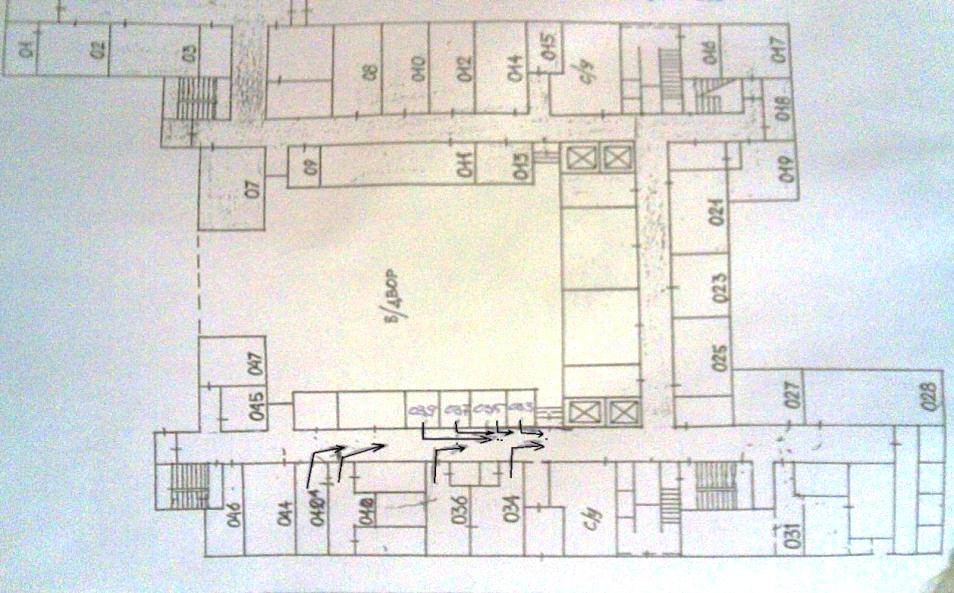
\includegraphics[width=0.6\textwidth]{schema_evacuation.png}
\caption{План евакуації}
\label{fig:schema_evacuation}
\end{figure}

На випадок пожежі в лабораторії є водопровід, вогнегасник вуглекислотно-брометиловий ОУБ-3 (ГОСТ~111564-65), а на сходових клітках і в коридорах шухляди з піском, вогнегасники ОХП-10, ОП-1Б та пожежні крани. Приміщення обладнане пожежною сигналізацією автоматичної дії комбінованого типу (оповісник~КИ-1).

Основними заходами по пожежній безпеці є регулярна перевірка працездатності засобів гасіння пожежі і систем пожежної сигналізації; перевірка справності електричної проводки; щорічне випробування опору ізоляції підвищеною напругою близько 500~В; обережне відношення з легкоплавкими речовинами.

\section{Висновки до розділу~\thechapter}

Були розглянуті шкідливі фактори, які присутні на місцях проведення дослідної роботи. Зважаючи на основні ДСТУ, ДСН, ДБН та СНиП, що регулюють необхідні для безпечної роботи параметри, було встановлено, що робоча лабораторія в якій проводилася НДР відповідає всім зазначеним нормам, окрім температурного режиму. Наведені приклади покращення.

\likechapter{ВИСНОВКИ}

Встановлена можливість створення функціональних покриттів товщиною від 15~мкм до 30~мкм на поверхні сталі~45 в процесі пошарового електроіскрового легування W-, Cr-, C-анодами.

Встановлено підвищення поверхневої мікротвердості сталі~45 у діапазоні від 11,5~ГПа до 18,9~ГПа після нанесення електроіскрових покриттів за всіма запропонованими схемами за рахунок наявності твердих розчинів матеріалів електродів та карбідів WC, W\textsubscript{2}C, Fe\textsubscript{3}C, Cr\textsubscript{3}C\textsubscript{2}, CrC.

Виявлено, що зносостійкість покриттів зростає в ряду C-Cr-W~$\rightarrow$~W-C-Cr~$\rightarrow$~W-Cr-C~$\rightarrow$~Cr-W-C у 2,9 разів та у 23~рази у порівнянні з необробленою поверхнею сталі~45. Найвищу зносостійкість має покриття Cr-W-C за рахунок наявності вільного графіту.

Для науково-дослідної роботи був розрахований коефіцієнт умовної економічної ефективності, який становить~1,02. З цього слідує, що проведення НДР є економічно доцільним.

Були розглянуті шкідливі фактори для здоров'я людини на місцях проведення науково-дослідної роботи. Таким чином було встановлено, що робоча лабораторія в якій проводилася НДР відповідає всім зазначеним нормам, окрім температурного режиму.

\bibliography{literature} % список литературы

\begin{appendices}
%\renewcommand\thechapter{\Asbuk{chapter}}
\setcounter{chapter}{0}

\append{ДІАГРАМИ СТАНУ}
\label{app:phase_diagrams}

\begin{figure}[h!]
\centering
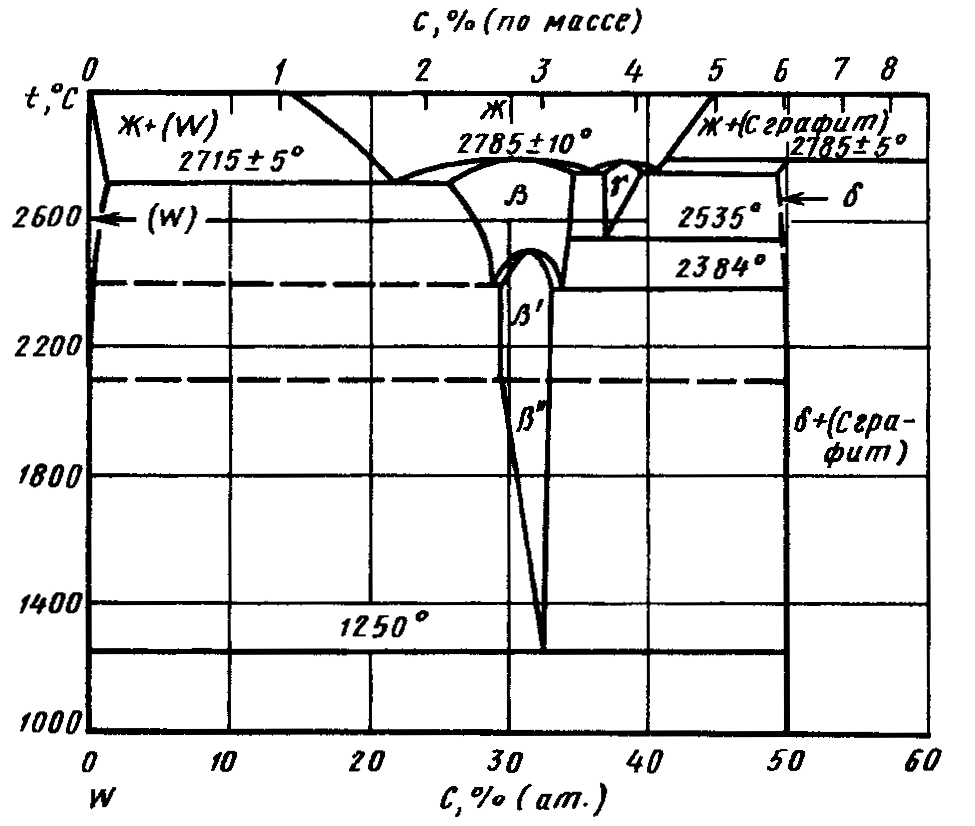
\includegraphics[width=0.9\textwidth]{C-W.png}
\caption{Діаграма стану системи C-W~\cite{diag1997t1}}
\label{fig:phase_diag_C-W}
\end{figure}

\begin{figure}[p!]
\centering
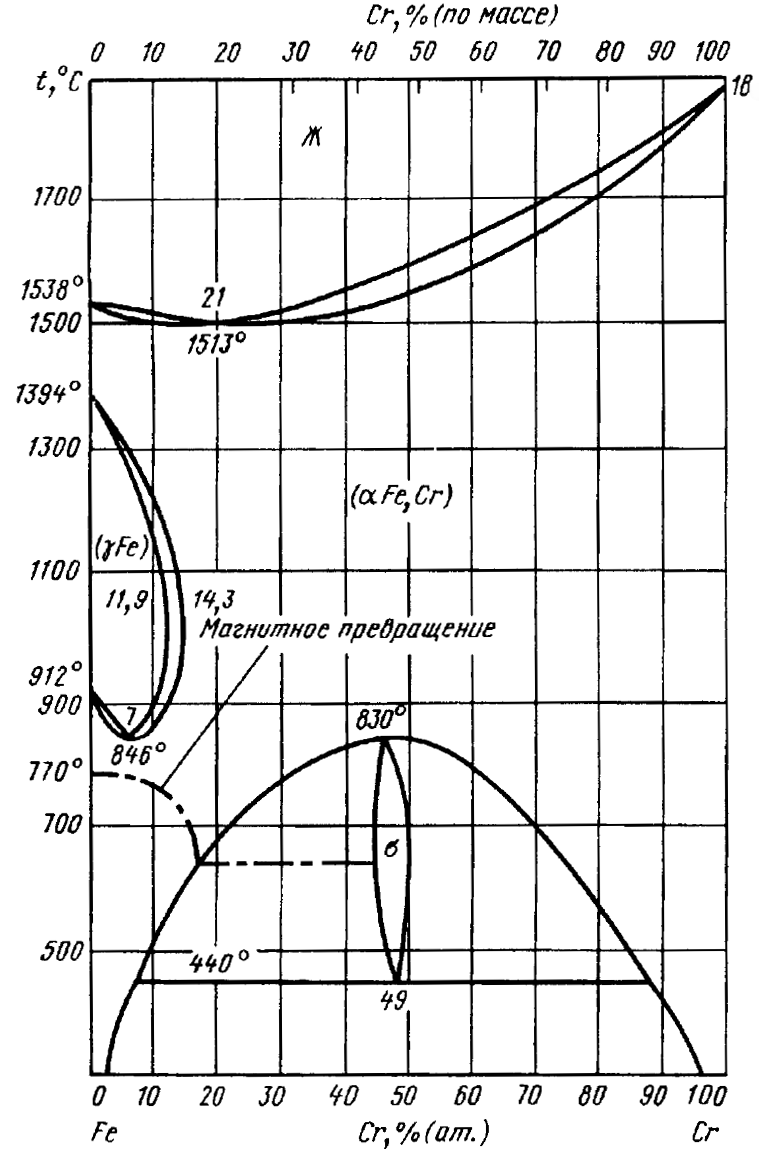
\includegraphics[width=0.9\textwidth]{Cr-Fe.png}
\caption{Діаграма стану системи Cr-Fe~\cite{diag1997t2}}
\label{fig:phase_diag_Cr-Fe}
\end{figure}

\append{ЛІСТИНГИ ВИКОНУЮЧИХ СКРИПТІВ}
\label{app:listings}
%\linespread{1} % вернем временно единичный межстрочный интервал
\lstinputlisting[%
language   = Python,
caption    = {Обробка фотографій мікроструктури (\lstname)},
label      = {list:microstructure}
]{./figures/ms.py}

\lstinputlisting[%
language   = Python,
caption    = {Гравіметричний аналіз (\lstname)},
label      = {list:grav}
]{./calc/grav.py}

\lstinputlisting[%
language   = Python,
caption    = {Мікродюрометричний аналіз },
label      = {list:hardness}
]{./calc/hardness.py}


% {% ДАНІ З RIGAKU ULTIMA IV
% % Зразок W-C-Cr
% \includepdf[scale=0.8,
% frame=true,
% offset=7mm -25mm,
% nup=1x2,
% delta=3mm 3mm,
% pagecommand={\fancyhead[R]{\thepage}\append{ДАНІ ПО РЕНТГЕНОФАЗОВОМУ АНАЛІЗУ} \vspace{-1cm}\section{Зразок W-C-Cr}\label{rigaku_W-C-Cr}},
% pages={1,2},
% ]{rigaku_W-C-Cr.pdf}
% \includepdf[scale=0.8,
% frame=true,
% offset=5mm 0mm,
% nup=1x2,
% delta=3mm 3mm,
% pagecommand={\fancyhead[R]{\thepage}},
% pages={3-4},
% ]{rigaku_W-C-Cr.pdf}

% % Зразок W-Cr-C
% \includepdf[scale=0.8,
% frame=true,
% offset=7mm -5mm,
% nup=1x2,
% delta=3mm 3mm,
% pagecommand={\fancyhead[R]{\thepage}\section{Зразок W-Cr-C}\label{rigaku_W-Cr-C}},
% pages={1,2},
% ]{rigaku_W-Cr-C.pdf}
% \includepdf[scale=0.8,
% frame=true,
% offset=5mm 0mm,
% nup=1x2,
% delta=3mm 3mm,
% pagecommand={\fancyhead[R]{\thepage}},
% pages={3-4},
% ]{rigaku_W-Cr-C.pdf}
%
% % Зразок C-Cr-W
% \includepdf[scale=0.8,
% frame=true,
% offset=7mm -5mm,
% nup=1x2,
% delta=3mm 3mm,
% pagecommand={\fancyhead[R]{\thepage}\section{Зразок C-Cr-W}\label{rigaku_C-Cr-W}},
% pages={1,2},
% ]{rigaku_C-Cr-W.pdf}
% \includepdf[scale=0.8,
% frame=true,
% offset=5mm 0mm,
% nup=1x2,
% delta=3mm 3mm,
% pagecommand={\fancyhead[R]{\thepage}},
% pages={3-4},
% ]{rigaku_C-Cr-W.pdf}
%
% % Зразок Cr-W-C
% \includepdf[scale=0.8,
% frame=true,
% offset=7mm -5mm,
% nup=1x2,
% delta=3mm 3mm,
% pagecommand={\fancyhead[R]{\thepage}\section{Зразок Cr-W-C}\label{rigaku_Cr-W-C}},
% pages={1,2},
% ]{rigaku_Cr-W-C.pdf}
% \includepdf[scale=0.8,
% frame=true,
% offset=5mm 0mm,
% nup=1x2,
% delta=3mm 3mm,
% pagecommand={\fancyhead[R]{\thepage}},
% pages={3-5},
% ]{rigaku_Cr-W-C.pdf}
% }

% {% МАТЕРІАЛИ ДОПОВІДІ
%   \includepdf[scale=0.7,
%     frame=true,
%     offset=7mm 0mm,
%     nup=1x2,
%     delta=3mm 3mm,
%     pagecommand={\fancyhead[R]{\thepage}\append{МАТЕРІАЛИ ДОПОВІДІ}},
%     pages={1,2},
%     ]{presentation/present.pdf}
%   \includepdf[scale=0.8,
%     frame=true,
%     offset=5mm 0mm,
%     nup=1x2,
%     delta=3mm 3mm,
%     pagecommand={\fancyhead[R]{\thepage}},
%     pages={3-14},
%     ]{presentation/present.pdf}
%}
\end{appendices}

%%%%%%%%%%%%%%%%%%%%%%%%%%%%%%%%%%%%%%%%%%%%%%%%%%%%%%%%%%%%%%%%%%%%%%%%%%%%%%%
\end{document}
